\documentclass[12pt]{article}

% -------------------------------------------------------------------
% Packages
% -------------------------------------------------------------------
\usepackage[margin=1in]{geometry}
\usepackage{amsmath,amssymb,amsthm}
\usepackage{hyperref}
\usepackage[authoryear,round]{natbib}
\usepackage{booktabs}
\usepackage{graphicx}
\usepackage{setspace}
\usepackage{enumitem}
\usepackage{float}

\onehalfspacing

% -------------------------------------------------------------------
% Theorem environments
% -------------------------------------------------------------------
\newtheorem{theorem}{Theorem}[section]
\newtheorem{proposition}[theorem]{Proposition}
\newtheorem{lemma}[theorem]{Lemma}
\newtheorem{corollary}[theorem]{Corollary}
\newtheorem{definition}[theorem]{Definition}
\newtheorem{assumption}[theorem]{Assumption}
\newtheorem{remark}[theorem]{Remark}

% -------------------------------------------------------------------
% Hyperref setup
% -------------------------------------------------------------------
\hypersetup{
  colorlinks=true,
  linkcolor=blue!70!black,
  citecolor=blue!70!black,
  urlcolor=blue!70!black
}

% -------------------------------------------------------------------
% Graphics path
% -------------------------------------------------------------------
\graphicspath{{../results/figures/}}

% -------------------------------------------------------------------
% Title
% -------------------------------------------------------------------
\title{A Theory of Endogenous Premium in Bitcoin Treasury Vehicles:\\
Accumulation Options, Reflexive Equilibria, and Capital Stack Dynamics}
\author{Haiyang Yu\thanks{UCLA Anderson School of Management.
  Email: \texttt{haiyang.yu@anderson.ucla.edu}.}}
\date{March 2026}

% ===================================================================
\begin{document}
% ===================================================================

\maketitle

%!TEX root = ../main.tex

\begin{abstract}
We develop a theory of endogenous premium formation for Bitcoin treasury
vehicles---publicly traded firms that hold BTC as their primary asset and
issue securities to fund ongoing accumulation.  The NAV premium equals the
present value of a \emph{perpetual accumulation option}: the right to issue
equity at a premium and purchase BTC, thereby increasing BTC-per-share for
existing holders.  The fair premium satisfies a fixed-point equation with a
closed-form steady-state approximation that links it to BTC volatility,
issuance intensity, leverage, and discount rates.  Reflexive feedback between
the premium and accumulation creates multiple equilibria---a high-premium
``flywheel,'' an unstable tipping point, and a low-premium ``death
spiral''---connected by saddle-node bifurcations exhibiting hysteresis.  We
reinterpret five structural indicators (ILE, TEE, PMRI, IBGR, IFRD) as
option Greeks of the embedded accumulation claim: Delta, Adjusted Delta,
Theta, Moneyness, and Exercise Cost.  We derive optimal capital structure
rules governing the transition from ATM equity to convertible debt to
preferred stock as the premium declines, and introduce the Weighted Average
Cost of BTC Acquisition (WACBA).  Market impact analysis yields a reflexivity
amplification factor and conditions for contagion cascades under corporate BTC
adoption.  Calibrating the model to Strategy (ticker: MSTR)---which holds
761,068~BTC (\$56.25B) as of March~2026---we estimate an OU premium process
with mean-reversion speed $\hat\kappa = 5.21$, long-run mean
$\hat\theta = 1.08$, and BTC volatility $\hat\sigma_S = 48.6\%$.  The
current premium of 24.2\% sits below its long-run mean
($\text{PMRI} = -0.71$), implying positive carry and an underpriced
accumulation option.  Three-year survival probability is 91.9\%, and the
implied funding requirement averages \$35.3B.  The framework provides a
unified lens for valuation, risk assessment, and vehicle selection (MSTR vs.\
BTC~ETF).

\medskip
\noindent\textbf{Keywords:} Bitcoin, NAV premium, accumulation option,
reflexivity, multiple equilibria, capital structure, Strategy (MSTR).

\noindent\textbf{JEL Codes:} G12, G13, G32, G23.
\end{abstract}


\newpage
%!TEX root = ../main.tex

\section{Introduction}\label{sec:introduction}

Strategy Incorporated (ticker: MSTR) holds 761,068 Bitcoin---approximately
3.8\% of the circulating supply---valued at \$56.25 billion as of March~2026.
Its equity trades at a persistent premium to net asset value: the market
capitalisation exceeds the mark-to-market value of the BTC holdings minus
liabilities.  This premium, which has ranged from near zero to over 200\%,
represents one of the most striking pricing anomalies in modern corporate
finance.  Yet no structural theory explains \emph{what} the fair premium
should be, \emph{when} it is justified, or \emph{how} it interacts with the
firm's capital structure decisions.

This paper fills the gap.  We develop a theory in which the NAV premium
is endogenous: it equals the present value of a \emph{perpetual accumulation
option}---the right to issue equity at a premium to NAV and deploy the
proceeds to purchase BTC, thereby increasing BTC-per-share for existing
holders.  The key insight is that this option is self-referential: the premium
that justifies the option is itself sustained by the option's value.  This
reflexive structure generates rich equilibrium dynamics, including multiple
stable equilibria and path-dependent transitions.

\paragraph{Contributions.}
The paper makes five contributions to the literature on alternative-asset
holding companies and crypto-finance:

\begin{enumerate}[leftmargin=*]
  \item \textbf{Endogenous premium theory with reflexivity.}
    We derive a fixed-point equation for the fair premium
    $\pi^\star$ that links it to BTC volatility, issuance intensity,
    leverage, and discount rates (Proposition~\ref{prop:fair_premium},
    Proposition~\ref{prop:steady_state}).  The closed-form steady-state
    approximation connects to the Black--Scholes call-option formula,
    providing both analytical tractability and economic intuition.

  \item \textbf{Multiple equilibria and death spiral.}
    The reflexive feedback loop creates three equilibria: a high-premium
    ``flywheel'' (virtuous cycle of issuance and accumulation), an unstable
    tipping point, and a low-premium spiral
    (Theorem~\ref{thm:three_equilibria}).  Transitions between equilibria
    exhibit hysteresis via saddle-node bifurcations
    (Proposition~\ref{prop:hysteresis}), and we characterise the death
    spiral mechanism formally (Theorem~\ref{thm:death_spiral}).

  \item \textbf{Greeks reinterpretation.}
    We show that five structural indicators---Implied Leverage Elasticity
    (ILE), Total Equity Elasticity (TEE), Premium Mean-Reversion Index
    (PMRI), Implied BTC Growth Rate (IBGR), and Implied Funding
    Requirement Distribution (IFRD)---map precisely onto the option Greeks
    of the embedded accumulation claim: Delta, Adjusted Delta, Theta,
    Moneyness, and Exercise Cost (Table~\ref{tab:greek-map}).  We further
    introduce Vega and Rho as new sensitivity measures.

  \item \textbf{Optimal capital structure.}
    We derive a premium-dependent financing rule that determines the
    cost-minimising channel among ATM equity, convertible debt, and
    preferred stock as a function of the log-premium
    (Proposition~\ref{prop:optimal_channel}).  We introduce the Weighted
    Average Cost of BTC Acquisition (WACBA) and characterise endogenous
    procyclical leverage dynamics (Proposition~\ref{prop:procyclical}).
    Strategy's observed financing behaviour---shifting from equity to
    convertibles to preferred stock as the premium declined through
    2025--2026---closely matches the model's predictions.

  \item \textbf{Empirical calibration through 2026.}
    We calibrate the model to a comprehensive daily panel of BTC prices,
    MSTR equity data, holdings, debt, and five series of preferred stock
    (STRK, STRF, STRC, STRD, STRE).  The calibrated premium process has
    mean-reversion speed $\hat\kappa = 5.21$ and long-run mean
    $\hat\theta = 1.08$, with BTC volatility of 48.6\%.  The current
    premium of 24.2\% sits well below the long-run mean
    ($\text{PMRI} = -0.71$), implying positive carry.
    Monte Carlo simulation with 5,000 paths yields a 91.9\% three-year
    survival probability, mean implied funding requirement of \$35.3B, and
    preferred dividend coverage ratio of $49\times$ currently.
\end{enumerate}

\paragraph{Broader implications.}
The framework applies beyond MSTR to any corporate treasury vehicle that
holds a volatile asset and issues securities to fund accumulation---including
the growing cohort of public companies adding BTC to their balance sheets.
Our market impact analysis (Section~\ref{sec:market_impact_theory})
formalises the systemic risk from corporate BTC concentration and derives
conditions for contagion cascades among leveraged holders.

\paragraph{Outline.}
Section~\ref{sec:literature} reviews related literature.
Section~\ref{sec:theory} develops the theoretical framework:
the accumulation option (Section~\ref{sec:fair_premium}),
reflexivity and multiple equilibria (Section~\ref{sec:multiple_equilibria}),
indicators as Greeks (Section~\ref{sec:greeks}),
MSTR vs.\ BTC ETF comparison (Section~\ref{sec:etf_comparison}),
optimal capital structure (Section~\ref{sec:optimal_capital}),
and market impact (Section~\ref{sec:market_impact_theory}).
Section~\ref{sec:empirical} describes the data and estimation.
Section~\ref{sec:results} presents calibrated results.
Section~\ref{sec:discussion} discusses implications and limitations.
Section~\ref{sec:conclusion} concludes.

%!TEX root = ../main.tex

\section{Related Literature}\label{sec:literature}

This paper connects to several strands of the finance literature.

\paragraph{Structural credit models.}
The structural approach to corporate liabilities originates with
\citet{merton1974pricing}, who models equity as a call option on the firm's
assets.  \citet{leland1994corporate} extends this framework to incorporate
endogenous default boundaries and optimal capital structure, while
\citet{leland1996optimal} adds debt maturity choice.  Our model shares the
structural perspective---MSTR equity is a levered claim on BTC---but
introduces an accumulation option absent from classical models, where asset
dynamics are exogenous.

\paragraph{Closed-end fund premia and discounts.}
The persistent deviation of closed-end fund (CEF) prices from NAV is a
well-documented anomaly.  \citet{lee1991investor} attribute discounts to
investor sentiment; \citet{pontiff1995closed} emphasises managerial expenses
and dividend policy; \citet{cherkes2009closed} model premia as reflecting
liquidity benefits.  The BTC treasury vehicle resembles a CEF in that equity
trades at a premium to the underlying asset value, but differs fundamentally:
the premium is sustained by an \emph{active} accumulation strategy rather
than passive holding, and the manager can issue new shares to grow the asset
base---a feature absent from standard CEFs.

\paragraph{Convertible securities and hybrid capital.}
The valuation of convertible bonds follows \citet{tsiveriotis1998valuing},
who decompose the instrument into equity and debt components.
\citet{brennan1977convertible} and \citet{ingersoll1977contingent} develop
structural models for convertible pricing.  Strategy's capital stack---common
equity, convertible notes, convertible preferred (STRK), and
non-convertible preferred (STRF, STRC, STRD, STRE)---creates a layered
priority structure that we model explicitly.  The interaction between
preferred dividends and common equity accumulation dynamics is novel.

\paragraph{Reflexivity and feedback in financial markets.}
\citet{soros1987alchemy} introduces the concept of reflexivity---the
feedback between market prices and the fundamentals they are supposed to
reflect.  In formal models, \citet{brunnermeier2014macroeconomic} and
\citet{he2013intermediary} study feedback loops between asset prices and
financial intermediary balance sheets.  \citet{brunnermeier2009market}
formalise margin spirals where declining collateral values trigger forced
sales.  Our reflexive flywheel mechanism is distinct: it operates through
\emph{voluntary} equity issuance at a premium rather than forced
deleveraging, though the death spiral shares features with margin spirals.

\paragraph{Cryptocurrency finance.}
The theoretical literature on cryptocurrency markets is growing rapidly.
\citet{biais2023equilibrium} model Bitcoin as a coordination game with
multiple equilibria in adoption.  \citet{cong2021tokenomics} develop a
dynamic model of token-based platforms.  \citet{foley2019sex} and
\citet{makarov2020trading} study Bitcoin market microstructure and
arbitrage.  On the empirical side, \citet{liu2021risks} document
cryptocurrency risk factors, and \citet{griffin2020bitcoin} examine price
manipulation.  Our contribution is orthogonal: we model the \emph{corporate
vehicle} that holds Bitcoin rather than the cryptocurrency itself, though
the market impact analysis (Section~\ref{sec:market_impact_theory}) connects
the two through the price feedback channel.

\paragraph{Bitcoin ETFs and passive vehicles.}
The approval of spot Bitcoin ETFs in the United States in January~2024
created a benchmark for pure delta-one BTC exposure.
\citet{alexander2024bitcoin} study ETF premium dynamics and the
creation/redemption mechanism.  We provide a formal comparison between the
ETF (zero accumulation option) and the treasury vehicle (positive
accumulation option), deriving conditions under which each dominates
(Section~\ref{sec:etf_comparison}).

\paragraph{Gap in the literature.}
No existing work provides a structural theory for the NAV premium of a BTC
treasury vehicle.  The CEF literature treats premia as anomalies driven by
sentiment or frictions; the structural credit literature assumes exogenous
asset dynamics; and the crypto-finance literature focuses on token design
and market microstructure.  Our paper bridges these literatures by showing
that the premium is the equilibrium price of an accumulation option whose
value depends endogenously on the premium itself.

%!TEX root = ../main.tex

\section{Theory}\label{sec:theory}

This section develops the theoretical framework.  We begin with the model
setup (Section~\ref{sec:setup}), derive the accumulation option and fair
premium (Section~\ref{sec:fair_premium}), analyse reflexivity and multiple
equilibria (Section~\ref{sec:multiple_equilibria}), reinterpret structural
indicators as option Greeks (Section~\ref{sec:greeks}), compare MSTR equity
to a BTC ETF (Section~\ref{sec:etf_comparison}), derive optimal capital
structure rules (Section~\ref{sec:optimal_capital}), and model market impact
and systemic risk (Section~\ref{sec:market_impact_theory}).

%=============================================================================
\subsection{Model Setup}\label{sec:setup}
%=============================================================================

We work on a filtered probability space
$(\Omega,\mathcal{F},(\mathcal{F}_t)_{t\ge 0},\mathbb{P})$ with the
following state variables:
\begin{itemize}
  \item $S_t$: BTC spot price;
  \item $H_t$: BTC holdings (in BTC);
  \item $D_t$: outstanding debt (face value);
  \item $N_t^{\mathrm{sh}}$: shares outstanding;
  \item $B_t = H_t / N_t^{\mathrm{sh}}$: BTC per share;
  \item $\mathrm{NAV}_t = (H_t S_t - D_t - P_t^{\mathrm{liq}})^+$: net asset
        value, where $P_t^{\mathrm{liq}}$ is the preferred stock liquidation
        value;
  \item $E_t = e^{\pi_t}\,\mathrm{NAV}_t$: equity market capitalisation;
  \item $\pi_t = \log(E_t / \mathrm{NAV}_t)$: log-premium to NAV.
\end{itemize}

We collect the observable state into the vector
\begin{equation}
  \label{eq:state_vector}
  \Phi_t = (S_t,\, H_t,\, D_t,\, N_t^{\mathrm{sh}},\, \sigma_S,\, \kappa,\, \alpha),
\end{equation}
where $\sigma_S$ is BTC volatility and $\alpha$ and $\kappa$ are behavioural
parameters defined below.

\begin{assumption}[Operating regime]
  \label{ass:operating_regime}
  We assume $A_t = H_t S_t > D_t + P_t^{\mathrm{liq}}$ so that
  $\mathrm{NAV}_t > 0$ and the log-premium $\pi_t$ is well-defined.
  The distress regime $A_t \le D_t + P_t^{\mathrm{liq}}$ is treated
  in Section~\ref{sec:death_spiral}.
\end{assumption}

\begin{assumption}[Equity issuance technology]
  \label{ass:issuance}
  The firm can issue new shares at-the-market at the prevailing equity price
  $P_t$ and immediately deploy the proceeds to purchase BTC at price $S_t$.
  Issuance is frictionless up to a market-impact cost parameterised by
  $\eta \ge 0$.
\end{assumption}

%=============================================================================
\subsection{The Accumulation Option and Fair Premium}\label{sec:fair_premium}
%=============================================================================

%-----------------------------------------------------------------------------
\subsubsection{Endogenous Premium System}\label{sec:coupled_system}
%-----------------------------------------------------------------------------

We replace an exogenous premium process with a \emph{coupled} system.

\begin{definition}[Endogenous premium system]
  \label{def:coupled_sdes}
  The joint dynamics of $(S_t, \pi_t, H_t)$ under $\mathbb{P}$ are:
  \begin{align}
    \frac{dS_t}{S_{t^-}} &= \mu_S\,dt + \sigma_S\,dW_t^S
      + \eta\,\frac{dH_t}{H_{t^-}},
    \label{eq:btc_impact} \\[6pt]
    d\pi_t &= \kappa\bigl(\pi^\star(\Phi_t) - \pi_t\bigr)\,dt
      + \sigma_\pi\,dW_t^\pi,
    \label{eq:premium_endo} \\[6pt]
    dH_t &= \alpha\,\pi_t^+\,dt + dH_t^{\mathrm{jump}},
    \label{eq:holdings_endo}
  \end{align}
  where $\mu_S$ is the BTC drift, $\eta \ge 0$ is market-impact elasticity,
  $\pi^\star(\Phi_t)$ is the endogenous fair premium derived below,
  $\alpha > 0$ governs continuous accumulation intensity,
  $\pi_t^+ = \max(\pi_t,0)$,
  $dH_t^{\mathrm{jump}} = \sum_k \Delta H_{\tau_k}\,\delta(t - \tau_k)$
  captures discrete financing events with Poisson arrival rate $\lambda_M$,
  and $\mathrm{corr}(dW_t^S, dW_t^\pi) = \rho$.
\end{definition}

\begin{remark}
  Setting $\pi^\star(\Phi_t) \equiv \theta$ (constant) recovers the exogenous
  OU premium process of the baseline model.
\end{remark}

The key novelty is that $\pi^\star$ depends on $\Phi_t$, creating a
\emph{feedback loop}:
\begin{equation}
  \label{eq:feedback_loop}
  \pi_t \uparrow \;\Longrightarrow\;
  H_t \uparrow \;\Longrightarrow\;
  B_t \uparrow \;\Longrightarrow\;
  \pi^\star \uparrow \;\Longrightarrow\;
  \pi_t \uparrow \;\cdots
\end{equation}
This is the \emph{reflexive flywheel} that distinguishes a BTC treasury
vehicle from a passive fund.

%-----------------------------------------------------------------------------
\subsubsection{Accretive Issuance: Single-Round Mechanics}
\label{sec:single_round}
%-----------------------------------------------------------------------------

\begin{definition}[Accretion from a single issuance]
  \label{def:single_accretion}
  Suppose the firm has $H$ BTC, $N$ shares, and trades at premium $\pi > 0$.
  It issues $\delta N$ new shares at market price
  $P = e^\pi \cdot (HS - D)/N$, raising proceeds to purchase
  $\delta H = e^\pi(HS-D)\delta N / (NS)$ BTC.  The change in BTC-per-share
  is
  \begin{equation}
    \label{eq:accretion_single}
    \frac{\Delta B}{B}
    = \frac{(e^\pi - 1)\,(1 - D/(HS))}{1 + \delta N / N}\cdot
      \frac{\delta N}{N}.
  \end{equation}
\end{definition}

For small issuance ($\delta N / N \ll 1$):
\begin{equation}
  \label{eq:accretion_approx}
  \frac{\Delta B}{B} \approx (e^\pi - 1)\,\frac{\delta N}{N}.
\end{equation}
Each round at $\pi > 0$ is BTC-per-share accretive.  At $\pi < 0$,
issuance is dilutive, so the firm optimally refrains: this is the
option-like payoff.

%-----------------------------------------------------------------------------
\subsubsection{Perpetual Accumulation Option Value}
\label{sec:vacc}
%-----------------------------------------------------------------------------

\begin{definition}[Accumulation option value]
  \label{def:vacc}
  The \emph{accumulation option value} is the present value of all future
  BTC-per-share accretion from optimally timed issuance:
  \begin{equation}
    \label{eq:vacc_def}
    V_{\mathrm{acc}}(\Phi_t)
    = \mathrm{NAV}_t \cdot
      \mathbb{E}^{\mathbb{P}}\!\left[
        \int_t^\infty e^{-r(u-t)}\,
        g(\pi_u,\Phi_u)\,du
        \;\Big|\;\mathcal{F}_t
      \right],
  \end{equation}
  where $r > 0$ is the discount rate and the accretion rate function is
  \begin{equation}
    \label{eq:accretion_rate}
    g(\pi,\Phi)
    = \alpha_N\,(e^\pi - 1)^+\,\biggl(1 - \frac{D}{HS}\biggr)^{\!+},
  \end{equation}
  with $\alpha_N > 0$ the issuance intensity (shares issued per unit time
  as a fraction of $N$).
\end{definition}

The $(e^\pi - 1)^+$ term captures the option-like feature: the firm issues
only when $\pi > 0$.

\begin{proposition}[Fair premium]
  \label{prop:fair_premium}
  Under the endogenous premium framework, the fair log-premium satisfies
  \begin{equation}
    \label{eq:pi_star_def}
    \boxed{
      \pi^\star(\Phi_t)
      = \log\!\left(1 + \frac{V_{\mathrm{acc}}(\Phi_t)}{\mathrm{NAV}_t}\right).
    }
  \end{equation}
\end{proposition}

\begin{proof}
  In equilibrium, $E_t = \mathrm{NAV}_t + V_{\mathrm{acc}}(\Phi_t)$.
  Since $E_t = e^{\pi_t}\,\mathrm{NAV}_t$, setting $\pi_t = \pi^\star$:
  \[
    e^{\pi^\star}\,\mathrm{NAV}_t = \mathrm{NAV}_t + V_{\mathrm{acc}},
  \]
  which gives~\eqref{eq:pi_star_def}.
\end{proof}

\begin{remark}
  $\pi^\star > 0$ if and only if $V_{\mathrm{acc}} > 0$.  A passive BTC
  holding company with no issuance capability ($\alpha_N = 0$) has
  $V_{\mathrm{acc}} = 0$ and thus $\pi^\star = 0$: it should trade at NAV.
\end{remark}

%-----------------------------------------------------------------------------
\subsubsection{Steady-State Closed-Form Approximation}
\label{sec:steady_state}
%-----------------------------------------------------------------------------

\begin{assumption}[Steady-state approximation]
  \label{ass:steady_state}
  The premium $\pi_t$ fluctuates around $\pi^\star$ as a stationary OU
  process with speed $\kappa$ and volatility $\sigma_\pi$.  The state
  variables $(S_t, H_t, D_t)$ evolve slowly relative to premium
  mean-reversion.
\end{assumption}

Under this assumption, $\pi \sim \mathcal{N}(\pi^\star, (\sigma_\pi^{\mathrm{ss}})^2)$
where $\sigma_\pi^{\mathrm{ss}} = \sigma_\pi / \sqrt{2\kappa}$.

\begin{proposition}[Steady-state fair premium]
  \label{prop:steady_state}
  With leverage ratio $\ell = D/(HS)$ and $L = (1-\ell)^+$, the fair
  premium satisfies the fixed-point equation
  \begin{equation}
    \label{eq:pi_star_fp}
    \pi^\star
    = \log\!\left(
        1 + \frac{\alpha_N L}{r}\,
        \mathbb{E}\bigl[(e^{\pi} - 1)^+\bigr]
      \right),
  \end{equation}
  where $\pi \sim \mathcal{N}(\pi^\star,\, (\sigma_\pi^{\mathrm{ss}})^2)$.
  Evaluating the expectation:
  \begin{equation}
    \label{eq:pi_star_closed}
    \boxed{
      \pi^\star
      = \log\!\left(
          1 + \frac{\alpha_N L}{r}\,\Bigl[
            e^{\pi^\star + (\sigma_\pi^{\mathrm{ss}})^2/2}\,
            \Phi\!\left(\frac{\pi^\star}{\sigma_\pi^{\mathrm{ss}}}
              + \sigma_\pi^{\mathrm{ss}}\right)
            - \Phi\!\left(\frac{\pi^\star}{\sigma_\pi^{\mathrm{ss}}}\right)
          \Bigr]
        \right),
    }
  \end{equation}
  where $\Phi(\cdot)$ is the standard normal CDF.
\end{proposition}

\begin{proof}
  At steady state, $V_{\mathrm{acc}}/\mathrm{NAV} = (\alpha_N L / r)\,
  \mathbb{E}[(e^\pi - 1)^+]$.  The expectation with
  $\pi \sim \mathcal{N}(m, v^2)$ is the Black--Scholes formula at strike
  $K=1$:
  \[
    \mathbb{E}[(e^\pi - 1)^+]
    = e^{m + v^2/2}\,\Phi\!\left(\frac{m}{v} + v\right)
      - \Phi\!\left(\frac{m}{v}\right),
  \]
  with $m = \pi^\star$, $v = \sigma_\pi^{\mathrm{ss}}$.
  Substituting into~\eqref{eq:pi_star_def} yields~\eqref{eq:pi_star_closed}.
\end{proof}

%-----------------------------------------------------------------------------
\subsubsection{Comparative Statics}\label{sec:comparative_statics}
%-----------------------------------------------------------------------------

\begin{proposition}[Comparative statics of the fair premium]
  \label{prop:comp_statics}
  Let $F(\pi^\star;\,\sigma_S,\kappa,\alpha_N,\ell,r)$ denote the
  right-hand side of~\eqref{eq:pi_star_closed}.  At any interior fixed point
  $\pi^\star > 0$ with $\partial F/\partial \pi^\star < 1$ (stable
  equilibrium):
  \begin{enumerate}
    \item $\partial \pi^\star / \partial \sigma_S > 0$:
      higher BTC volatility increases the option value of future accretive
      issuance.
    \item $\partial \pi^\star / \partial \kappa < 0$:
      faster mean-reversion reduces stationary variance and hence option
      value.
    \item $\partial \pi^\star / \partial \alpha_N > 0$:
      greater issuance ability increases option value (the IBGR channel).
    \item $\partial \pi^\star / \partial \ell < 0$ for $\ell < 1$:
      higher leverage reduces accretion efficiency.
    \item $\partial \pi^\star / \partial r < 0$:
      higher discount rates reduce present value of future accretion.
  \end{enumerate}
\end{proposition}

\begin{proof}
  By the implicit function theorem at a fixed point with $F_{\pi^\star} < 1$:
  $\partial \pi^\star / \partial p_i = (\partial F/\partial p_i) /
  (1 - \partial F / \partial \pi^\star)$.
  The denominator is positive at a stable equilibrium.  The signs of the
  numerators follow from direct differentiation
  of~\eqref{eq:pi_star_closed}: (1)~the Black--Scholes call value has
  positive vega; (2)~$\sigma_\pi^{\mathrm{ss}}$ is decreasing in $\kappa$;
  (3)~$F$ is increasing in $\alpha_N$; (4)~$L = (1-\ell)^+$ is decreasing
  in $\ell$; (5)~$r$ appears in the denominator.
\end{proof}

\begin{corollary}[Conditions for positive fair premium]
  \label{cor:sign_pistar}
  $\pi^\star > 0$ if and only if $\alpha_N > 0$, $L > 0$ (i.e.\
  $\ell < 1$), and $\sigma_\pi^{\mathrm{ss}} > 0$.
  A passive holding company ($\alpha_N = 0$) or one at maximum leverage
  ($\ell \ge 1$) has $\pi^\star = 0$.
\end{corollary}

%=============================================================================
\subsection{Reflexivity and Multiple Equilibria}
\label{sec:multiple_equilibria}
%=============================================================================

%-----------------------------------------------------------------------------
\subsubsection{Feedback Gain}\label{sec:feedback_gain}
%-----------------------------------------------------------------------------

\begin{definition}[Feedback gain]
  \label{def:feedback_gain}
  The feedback gain at equilibrium $\pi^\star$ is
  \begin{equation}
    \label{eq:feedback_gain}
    G(\pi^\star)
    = \frac{\partial F}{\partial \pi^\star},
  \end{equation}
  measuring the marginal increase in the fair premium from a unit increase
  in the current premium level.
\end{definition}

\begin{proposition}[Effective mean-reversion]
  \label{prop:effective_kappa}
  Near a stable equilibrium with feedback gain $G < 1$, the effective
  mean-reversion speed is
  \begin{equation}
    \label{eq:kappa_eff}
    \boxed{
      \kappa_{\mathrm{eff}} = \kappa\,(1 - G).
    }
  \end{equation}
\end{proposition}

\begin{proof}
  Linearise $\pi^\star(\Phi_t)$ around steady state.  When $\pi_t$ increases
  by $\delta\pi$, the target shifts by $G\,\delta\pi$.  The restoring drift
  becomes $-\kappa(1 - G)\,\delta\pi$.
\end{proof}

Three regimes emerge: (i)~$G < 1$: stable, premium mean-reverts more slowly
than the exogenous model; (ii)~$G = 1$: critical, mean-reversion vanishes;
(iii)~$G > 1$: unstable, perturbations self-amplify.

%-----------------------------------------------------------------------------
\subsubsection{Fixed-Point Analysis and Equilibrium Multiplicity}
\label{sec:fixed_point}
%-----------------------------------------------------------------------------

\begin{theorem}[Existence and multiplicity of equilibria]
  \label{thm:three_equilibria}
  Consider the fixed-point equation $\pi^\star = F(\pi^\star)$
  from~\eqref{eq:pi_star_closed} with parameters
  $(\alpha_N, L, r, \sigma_\pi^{\mathrm{ss}})$ all strictly positive.
  Define the feedback strength
  \begin{equation}
    \label{eq:feedback_strength}
    \Gamma = \frac{\alpha_N L}{r}.
  \end{equation}
  Then:
  \begin{enumerate}
    \item \textbf{Weak feedback:} If $\Gamma$ is sufficiently small, there
      exists a unique fixed point $\pi^\star_{\mathrm{low}} > 0$ (stable,
      $G < 1$).
    \item \textbf{Strong feedback:} If $\Gamma$ is sufficiently large,
      three fixed points exist:
      $\pi^\star_{\mathrm{low}}$ (stable),
      $\pi^\star_{\mathrm{mid}}$ (unstable tipping point, $G > 1$), and
      $\pi^\star_{\mathrm{high}}$ (stable flywheel).
    \item \textbf{Bifurcation:} The transition occurs at a critical
      $\Gamma^*$ via saddle-node bifurcation where
      $\pi^\star_{\mathrm{mid}}$ and $\pi^\star_{\mathrm{high}}$ collide.
  \end{enumerate}
\end{theorem}

\begin{proof}
  Define $h(\pi^\star) = F(\pi^\star) - \pi^\star$.  We have $h(0) > 0$
  (since $\sigma_\pi^{\mathrm{ss}} > 0$ implies positive option value at
  $\pi^\star = 0$).  For small $\Gamma$, $F' < 1$ everywhere, so $h$ is
  strictly decreasing with a unique zero.  For large $\Gamma$, the
  exponential growth of the option value creates a region where $F' > 1$,
  producing the S-shaped curve with three crossings.  At the critical
  $\Gamma^*$, $h(\pi^\star_c) = 0$ and $h'(\pi^\star_c) = 0$
  simultaneously---the standard saddle-node bifurcation.  Stability follows
  from $G < 1$ at the low and high equilibria and $G > 1$ at the middle.
\end{proof}

\begin{remark}[Economic interpretation]
  \label{rem:three_equil_econ}
  The \textbf{flywheel} ($\pi^\star_{\mathrm{high}}$): high premium $\to$
  aggressive issuance $\to$ rapid accretion $\to$ justified high premium.
  The \textbf{tipping point} ($\pi^\star_{\mathrm{mid}}$): unstable
  separator between basins of attraction.
  The \textbf{spiral} ($\pi^\star_{\mathrm{low}}$): low premium $\to$
  minimal issuance $\to$ negligible accretion $\to$ justified low premium.
\end{remark}

%-----------------------------------------------------------------------------
\subsubsection{Hysteresis}\label{sec:hysteresis}
%-----------------------------------------------------------------------------

\begin{proposition}[Hysteresis in premium transitions]
  \label{prop:hysteresis}
  Consider a parameter path where $\Gamma$ increases through $\Gamma^*$
  and then decreases.
  \begin{enumerate}
    \item As $\Gamma$ increases past $\Gamma^*$, the system at
      $\pi^\star_{\mathrm{low}}$ does not jump to
      $\pi^\star_{\mathrm{high}}$; it remains at the low equilibrium until
      a large shock exceeds the tipping point.
    \item If at $\pi^\star_{\mathrm{high}}$ and $\Gamma$ decreases below
      $\Gamma^*$, the flywheel equilibrium vanishes and the premium
      collapses discontinuously to $\pi^\star_{\mathrm{low}}$.
    \item The path exhibits hysteresis: the equilibrium depends on the
      direction of approach.
  \end{enumerate}
\end{proposition}

\begin{proof}
  Standard saddle-node bifurcation: when the stable (flywheel) and unstable
  (tipping) branches annihilate, no nearby attractor exists, forcing a
  discontinuous transition.
\end{proof}

%-----------------------------------------------------------------------------
\subsubsection{Death Spiral Mechanism}\label{sec:death_spiral}
%-----------------------------------------------------------------------------

\begin{theorem}[Death spiral]
  \label{thm:death_spiral}
  If $\pi_t < 0$ (discount to NAV):
  \begin{enumerate}
    \item $V_{\mathrm{acc}} \approx 0$ since issuance at a discount is
      dilutive and the firm refrains.
    \item The fair premium collapses to $\pi^\star \approx 0$.
    \item The feedback loop reverses:
      $\pi_t < 0 \Rightarrow \alpha_N^{\mathrm{eff}} = 0 \Rightarrow
      V_{\mathrm{acc}} \downarrow \Rightarrow \pi^\star \downarrow
      \Rightarrow \pi_t \downarrow$.
    \item A death spiral occurs when
      \begin{equation}
        \label{eq:spiral_condition}
        e^{\pi_t} < \frac{D_t}{H_t S_t}
        \quad\Longleftrightarrow\quad
        E_t < D_t,
      \end{equation}
      i.e.\ the market values equity below the debt burden.
  \end{enumerate}
\end{theorem}

\begin{proof}
  When $\pi_t \le 0$, $(e^\pi - 1)^+ = 0$, so $V_{\mathrm{acc}} = 0$ and
  $\pi^\star = 0$.  The natural OU restoring drift is
  $\kappa(0 - \pi_t) > 0$, tending toward recovery.  However, if forced
  dilutive issuance (to meet debt service) exceeds natural mean-reversion,
  the vicious cycle takes hold when $E_t < D_t$.
\end{proof}

%-----------------------------------------------------------------------------
\subsubsection{Mispricing Metric and Z-Score Bands}
\label{sec:mispricing}
%-----------------------------------------------------------------------------

\begin{definition}[Premium mispricing]
  \label{def:mispricing}
  The mispricing is $\Delta_t = \pi_t - \pi^\star(\Phi_t)$.
  Positive $\Delta_t$: overvaluation; negative: undervaluation.
\end{definition}

\begin{proposition}[Dynamics of the mispricing]
  \label{prop:delta_dynamics}
  Under the slow-variation assumption, $\Delta_t$ satisfies
  \begin{equation}
    \label{eq:delta_ou}
    d\Delta_t \approx -\kappa\,\Delta_t\,dt
      + \sigma_\pi\,dW_t^\pi
      - d\pi^\star(\Phi_t),
  \end{equation}
  with mispricing mean-reversion speed
  \begin{equation}
    \label{eq:kappa_delta}
    \boxed{
      \kappa_\Delta = \kappa > \kappa_{\mathrm{eff}}.
    }
  \end{equation}
  The mispricing reverts faster than the premium itself.
\end{proposition}

\begin{proof}
  Write $\pi_t = \pi^\star + \Delta_t$.  From~\eqref{eq:premium_endo},
  $d\pi_t = -\kappa\Delta_t\,dt + \sigma_\pi dW_t^\pi$.  Subtracting
  $d\pi^\star$: $d\Delta_t = -\kappa\Delta_t\,dt + \sigma_\pi dW_t^\pi
  - d\pi^\star$.  Since $\kappa > \kappa(1-G) = \kappa_{\mathrm{eff}}$
  for $G > 0$, the mispricing reverts faster.
\end{proof}

\begin{definition}[Mispricing Z-score]
  \label{def:zscore}
  \begin{equation}
    \label{eq:zscore}
    Z_t^{\Delta} = \frac{\Delta_t}{\sigma_\pi / \sqrt{2\kappa}}.
  \end{equation}
\end{definition}

Under the OU approximation, $Z_t^\Delta$ is approximately standard normal,
yielding classification bands: $|Z| < 1$ (fair value), $1$--$2$ (moderate
mispricing), $> 2$ (extreme mispricing, mean-reversion expected).

\begin{proposition}[Half-life of mispricing]
  \label{prop:halflife}
  $t_{1/2}^{\Delta} = \ln 2 / \kappa$, shorter than the premium half-life
  $\ln 2 / \kappa_{\mathrm{eff}}$ by the factor $(1-G)$.
\end{proposition}

%=============================================================================
\subsection{Structural Indicators as Option Greeks}\label{sec:greeks}
%=============================================================================

The structural relation $E_t = e^{\pi_t}(A_t - D_t - P_t^{\mathrm{liq}})^+$
endows MSTR equity with an option-like payoff on Bitcoin.  If $\pi_t$ encodes
the accumulation option value, then the structural indicators are precisely
the option Greeks of this embedded claim.

\begin{definition}[Accumulation option value]
  \label{def:acc_option_greeks}
  $V_{\mathrm{acc}}(t) = E_t - \mathrm{NAV}_t = (e^{\pi_t} - 1)(A_t - D_t - P_t^{\mathrm{liq}})^+$.
  When $\pi_t > 0$ the option is in the money; when $\pi_t \le 0$ it is
  worthless.
\end{definition}

%-----------------------------------------------------------------------------
\subsubsection{ILE as Delta}
%-----------------------------------------------------------------------------

\begin{proposition}[ILE $\equiv$ Leverage Delta]\label{prop:ile_delta}
  With $\pi_t$ held fixed:
  \begin{equation}
    \Delta_{\mathrm{lev}}(t)
    = \frac{\partial \log E_t}{\partial \log S_t}\bigg|_{\pi_t}
    = \frac{A_t}{A_t - D_t - P_t^{\mathrm{liq}}}
    = \mathrm{ILE}_t.
  \end{equation}
\end{proposition}

\begin{proof}
  $\log E_t = \pi_t + \log(H_tS_t - D_t - P_t^{\mathrm{liq}})$.
  Differentiating w.r.t.\ $\log S_t$ with $H_t, D_t, P_t^{\mathrm{liq}}$
  fixed gives $H_tS_t / (H_tS_t - D_t - P_t^{\mathrm{liq}}) = \mathrm{ILE}_t$.
\end{proof}

With calibrated values, $\mathrm{ILE}_0 = 1.49$: a 1\% BTC move produces a
1.49\% equity move from leverage alone.

%-----------------------------------------------------------------------------
\subsubsection{TEE as Adjusted Delta}
%-----------------------------------------------------------------------------

\begin{proposition}[TEE $\equiv$ Total Delta]\label{prop:tee_delta}
  Let $\gamma_{\pi S}$ denote the sensitivity of the log-premium to BTC
  log-returns.  Then
  \begin{equation}
    \Delta_{\mathrm{tot}}(t)
    = \frac{d\log E_t}{d\log S_t}
    = \gamma_{\pi S} + \mathrm{ILE}_t
    = \mathrm{TEE}_t.
  \end{equation}
\end{proposition}

\begin{proof}
  Total derivative: $d\log E_t / d\log S_t = d\pi_t/d\log S_t + A_t/(A_t - D_t - P_t^{\mathrm{liq}})$.
\end{proof}

At current calibration, $\mathrm{TEE}_0 = -3.60 + 1.49 = -2.11$: net equity
moves inversely to BTC, reflecting a regime where premium compression
dominates leverage.

%-----------------------------------------------------------------------------
\subsubsection{PMRI as Theta}
%-----------------------------------------------------------------------------

\begin{proposition}[PMRI $\equiv$ Premium Theta]\label{prop:pmri_theta}
  Under OU dynamics $d\pi_t = \kappa(\theta - \pi_t)\,dt + \sigma_\pi dW_t^\pi$,
  the standardised expected premium decay is
  \begin{equation}
    \Theta_\pi(t)
    = \frac{\pi_t - \theta}{\sigma_\pi / \sqrt{2\kappa}}
    = \mathrm{PMRI}_t.
  \end{equation}
\end{proposition}

With $\kappa = 5.21$, $\theta = 1.08$, $\sigma_\pi = 3.79$, and
$\pi_0 = 0.24$:
\[
  \sigma_{\mathrm{stat}} = \frac{3.79}{\sqrt{2 \times 5.21}} = 1.175,
  \quad
  \mathrm{PMRI}_0 = \frac{0.24 - 1.08}{1.175} = -0.71.
\]
The negative value implies the premium is below its long-run mean,
conferring positive expected carry.

%-----------------------------------------------------------------------------
\subsubsection{IBGR as Moneyness}
%-----------------------------------------------------------------------------

\begin{proposition}[IBGR $\equiv$ Moneyness]\label{prop:ibgr_moneyness}
  The implied BTC growth rate
  \begin{equation}
    \mathrm{IBGR}_t = \mu_H(t)
    = \frac{1}{H_t}\bigl(\alpha\,\pi_t^+ + \lambda_M\,\mathbb{E}[\Delta H]\bigr)
  \end{equation}
  measures how deeply in the money the accumulation option is.
\end{proposition}

With current calibration, $\mathrm{IBGR}_0 = (0 + 19.05 \times 7{,}044) /
761{,}068 = 17.6\%$ annualised.

%-----------------------------------------------------------------------------
\subsubsection{IFRD as Exercise Cost}
%-----------------------------------------------------------------------------

\begin{proposition}[IFRD $\equiv$ Exercise Cost]\label{prop:ifrd_strike}
  The implied funding requirement $G_T = \int_0^T S_u\,dH_u$ is the
  cumulative exercise cost of the accumulation option.  From simulation:
  $\mathbb{E}[G_{3\mathrm{y}}] = \$35.3$B, $G_{3\mathrm{y}}^{95\%} = \$71.8$B.
\end{proposition}

%-----------------------------------------------------------------------------
\subsubsection{Summary and New Greeks}
%-----------------------------------------------------------------------------

\begin{table}[H]
\centering
\caption{Structural indicators as option Greeks.}
\label{tab:greek-map}
\begin{tabular}{@{}llll@{}}
\toprule
\textbf{Indicator} & \textbf{Greek} & \textbf{Formula} & \textbf{Calibrated} \\
\midrule
ILE $= A/(A-D-P^{\mathrm{liq}})$ & Delta ($\Delta_{\mathrm{lev}}$)
  & $\partial\log E / \partial\log S\big|_\pi$
  & $1.49$ \\[4pt]
TEE $= \gamma_{\pi S} + \text{ILE}$ & Adjusted Delta ($\Delta_{\mathrm{tot}}$)
  & $d\log E / d\log S$
  & $-2.11$ \\[4pt]
PMRI $= (\pi-\theta)/\sigma_{\mathrm{stat}}$ & Theta ($\Theta_\pi$)
  & Premium carry cost
  & $-0.71$ \\[4pt]
IBGR $= \mu_H$ & Moneyness
  & $(\alpha\pi^+ + \lambda_M\mathbb{E}[\Delta H])/H$
  & $17.6\%$ \\[4pt]
IFRD $= G_T$ & Exercise cost
  & $\int S\,dH$
  & \$35.3B (mean) \\
\bottomrule
\end{tabular}
\end{table}

We introduce two additional Greeks absent from the original indicator set:

\begin{definition}[Premium Vega]
  $\mathcal{V}_\pi = \partial\pi^*/\partial\sigma_S$.
\end{definition}

\begin{proposition}[Positive Vega]\label{prop:vega}
  The accumulation option has $\mathcal{V}_\pi > 0$: higher BTC volatility
  increases the fair premium through option convexity and more frequent
  flywheel episodes.
\end{proposition}

\begin{proof}
  The equity payoff $(A_t - D_t)^+$ is convex in $S_t$ (Jensen's inequality),
  and higher $\sigma_S$ generates more accumulation opportunities through the
  drift $\alpha\pi_t^+$.
\end{proof}

\begin{definition}[Premium Rho]
  $\mathcal{R}_\pi = \partial\pi^*/\partial r$.
\end{definition}

\begin{proposition}[Negative Rho]\label{prop:rho_negative}
  $\mathcal{R}_\pi < 0$: higher interest rates decrease the fair premium
  through increased debt servicing cost, higher financing cost, and higher
  discount rate on future accretion.
\end{proposition}

%=============================================================================
\subsection{MSTR vs.\ BTC ETF: Premium Decomposition}
\label{sec:etf_comparison}
%=============================================================================

The launch of spot Bitcoin ETFs created a pure delta-one BTC exposure at
NAV.  Why does MSTR trade at a premium?

\begin{definition}[BTC ETF]\label{def:etf}
  A spot BTC ETF satisfies $E_t^{\mathrm{ETF}} = H_t^{\mathrm{ETF}}S_t$,
  with $\pi^{\mathrm{ETF}} = 0$, no debt, no leverage ($\mathrm{ILE} = 1$),
  no accumulation option, and $\Delta_{\mathrm{tot}}^{\mathrm{ETF}} = 1$.
\end{definition}

\begin{theorem}[Three-component premium decomposition]
  \label{thm:decomposition}
  The MSTR log-premium decomposes as
  \begin{equation}
    \pi_t
    = \underbrace{\pi_{\mathrm{lev}}(t)}_{\text{leverage}}
    + \underbrace{\pi_{\mathrm{acc}}(t)}_{\text{accumulation}}
    + \underbrace{\pi_{\mathrm{noise}}(t)}_{\text{residual}},
  \end{equation}
  where $\pi_{\mathrm{lev}} = \log(\mathrm{ILE}_t)$ and
  $\pi_{\mathrm{acc}} = \log(1 + V_{\mathrm{acc}}/\mathrm{NAV}_t)$.
\end{theorem}

\begin{proof}
  From $E_t = \mathrm{NAV}_t + V_{\mathrm{acc}} + \varepsilon_t$,
  taking logs: $\pi_t = \log(E_t/\mathrm{NAV}_t)$.  The leverage premium
  $\pi_{\mathrm{lev}} = \log(A_t/(A_t - D_t - P_t^{\mathrm{liq}}))$
  captures the excess sensitivity from the levered structure, the
  accumulation premium captures option value, and the residual absorbs
  sentiment and noise.
\end{proof}

At current calibration: $\pi_{\mathrm{lev}} = \log(1.488) = 0.398$ and
$\pi_0 - \pi_{\mathrm{lev}} = 0.242 - 0.398 = -0.156$, implying the
current premium does not fully compensate for leverage risk---the
accumulation option is priced at a discount.

\begin{proposition}[MSTR dominance conditions]\label{prop:mstr_dominates}
  MSTR offers superior risk-adjusted BTC exposure when:
  (i)~$\pi_{\mathrm{acc}} > 0$ (accumulation option in the money),
  (ii)~$\mathrm{PMRI}_t < 0$ (premium underpriced), and
  (iii)~$\mathrm{ILE}_t < \bar\beta$ (sustainable leverage).
\end{proposition}

\begin{proof}
  The expected MSTR excess return over the ETF is
  $\mathbb{E}[\Delta\pi_t] + (\mathrm{ILE}_t - 1)\mathbb{E}[\Delta\log S_t]$.
  Under conditions (i)--(iii), the first term is positive (premium expansion),
  the second provides leverage upside, and leverage risk is bounded.
\end{proof}

\begin{proposition}[ETF dominance conditions]\label{prop:etf_dominates}
  The ETF dominates when any of: $\mathrm{PMRI}_t > 0$ (overpriced premium),
  $\mathrm{ILE}_t > \bar\beta$ (excessive leverage),
  $\mathrm{IBGR}_t \le 0$ (stalled flywheel), or deteriorating dividend
  coverage.
\end{proposition}

\begin{corollary}[Premium regime map]\label{cor:regime_map}
  \begin{center}
  \begin{tabular}{@{}lcc@{}}
  \toprule
  & $\mathrm{IBGR} > 0$ & $\mathrm{IBGR} \le 0$ \\
  \midrule
  $\mathrm{PMRI} < 0$ (underpriced)
    & \textbf{MSTR dominates} & Transition / distress \\
  $\mathrm{PMRI} > 0$ (overpriced)
    & Hold / hedge & \textbf{ETF dominates} \\
  \bottomrule
  \end{tabular}
  \end{center}
  At current calibration ($\mathrm{IBGR} = 17.6\%$,
  $\mathrm{PMRI} = -0.71$), MSTR dominates.
\end{corollary}

\begin{table}[H]
\centering
\caption{MSTR vs.\ spot BTC ETF: structural comparison.}
\label{tab:mstr-vs-etf}
\begin{tabular}{@{}lcc@{}}
\toprule
\textbf{Metric} & \textbf{MSTR} & \textbf{BTC ETF} \\
\midrule
BTC Delta (ILE) & 1.49 & 1.00 \\
Total Delta (TEE) & $-2.11$ & 1.00 \\
Premium ($\pi$) & 0.24 (27\% over NAV) & $\approx 0$ \\
Accumulation option & In the money & None \\
IBGR (annualised) & 17.6\% & 0\% \\
Premium carry (PMRI) & $-0.71$ (positive carry) & N/A \\
Leverage risk & Moderate (ILE $< 2$) & None \\
3-year survival & 91.9\% & 100\% \\
Preferred dividend drag & \$977M/year & None \\
Funding requirement (3y) & \$35.3B mean & None \\
\bottomrule
\end{tabular}
\end{table}

%=============================================================================
\subsection{Optimal Capital Structure and Financing}\label{sec:optimal_capital}
%=============================================================================

Strategy employs five financing channels: ATM common equity, convertible
senior notes, and three classes of perpetual preferred stock.

%-----------------------------------------------------------------------------
\subsubsection{ATM Equity}
%-----------------------------------------------------------------------------

\begin{proposition}[ATM accretion threshold]\label{prop:atm_threshold}
  ATM equity issuance is BTC-per-share accretive if and only if
  \begin{equation}
    \label{eq:atm_accretive}
    \pi_t > \log(\mathrm{ILE}_t)
    = \log\!\left(\frac{H_t S_t}{H_t S_t - D_t - P_t^{\mathrm{liq}}}\right).
  \end{equation}
  When accretive, the marginal cost of BTC via ATM is negative (value-creating).
\end{proposition}

\begin{proof}
  Each new share at price $P_t$ purchases $P_t/S_t$ BTC.  Accretive iff
  $P_t/S_t > B_t$, i.e.\ $e^{\pi_t}(A_t - D_t - P_t^{\mathrm{liq}})/(N_tS_t) > H_t/N_t$,
  giving $e^{\pi_t} > A_t/(A_t - D_t - P_t^{\mathrm{liq}}) = \mathrm{ILE}_t$.
\end{proof}

With $\mathrm{ILE}_0 = 1.488$, the threshold is $\pi_t > 0.397$.  The
current premium $\pi_0 = 0.242$ is below this threshold, indicating ATM
issuance would be mildly dilutive---consistent with Strategy's observed
shift toward preferred stock issuance.

%-----------------------------------------------------------------------------
\subsubsection{Convertible Senior Notes}
%-----------------------------------------------------------------------------

A convertible note with coupon $c_j$, conversion price $K_j$, and maturity
$T_j$ has effective cost:
\begin{equation}
  \label{eq:conv_cost}
  k_{\mathrm{conv},j} = c_j + \frac{1}{T_j - t}\,
  \mathbb{E}^{\mathbb{P}}\!\left[
    \left(\frac{D_j}{K_j}\cdot\frac{B_{T_j}}{1 + D_j/(K_jN_{T_j}^{\mathrm{sh}})}
    - \frac{D_j}{S_{T_j}}\right)^{\!+}
    \cdot \frac{S_{T_j}}{D_j}
  \right].
\end{equation}
Strategy's convertibles carry a weighted average coupon of 0.42\%, making
them the cheapest debt channel.

%-----------------------------------------------------------------------------
\subsubsection{Preferred Stock}
%-----------------------------------------------------------------------------

For non-convertible preferred (STRF at 10\%, STRD at 10\%, STRE at 10\%,
STRC at 9.6\% initial / 11.5\% current), the cost is
$k_{\mathrm{pref},j} = d_j L_j / \text{Proceeds}_j$, yielding effective
costs of 10.7\%--12.5\%.  The convertible preferred STRK (8\%, conversion at
\$1,000) has effective cost approximately 10\% with conversion currently deep
out-of-the-money.  Total annual preferred dividend: \$976.6M.

%-----------------------------------------------------------------------------
\subsubsection{Optimal Financing Rule}
%-----------------------------------------------------------------------------

\begin{proposition}[Optimal channel selection]\label{prop:optimal_channel}
  The cost-minimising financing rule is:
  \begin{equation}
    \label{eq:optimal_channel}
    c^*(\pi_t) =
    \begin{cases}
      \text{ATM equity} & \text{if } \pi_t > \pi^*_{\mathrm{ATM}},
        \quad k_{\mathrm{ATM}} < 0, \\[4pt]
      \text{Convertible bonds} & \text{if } \pi^*_{\mathrm{conv}} < \pi_t
        \le \pi^*_{\mathrm{ATM}},
        \quad k_{\mathrm{conv}} \approx 0.4\text{--}2.3\%, \\[4pt]
      \text{Preferred stock} & \text{if } \pi_t \le \pi^*_{\mathrm{conv}},
        \quad k_{\mathrm{pref}} \approx 10\text{--}12.5\%.
    \end{cases}
  \end{equation}
\end{proposition}

Strategy's observed behaviour closely matches: massive ATM and convertible
issuance in Q4~2024 ($\pi_t \approx 1.5$--$2.0$), shift to STRK/STRF in
early 2025, then heavy STRC/STRD/STRE issuance in H2~2025--Q1~2026 as the
premium declined to 0.2--0.5.

%-----------------------------------------------------------------------------
\subsubsection{WACBA and Leverage Dynamics}
%-----------------------------------------------------------------------------

\begin{definition}[WACBA]\label{def:wacba}
  The Weighted Average Cost of BTC Acquisition:
  \begin{equation}
    \mathrm{WACBA}_t = \sum_{c \in \mathcal{C}} w_c(t)\, k_c(\pi_t, S_t),
  \end{equation}
  where $w_c(t)$ is the share of BTC acquired through channel $c$.
\end{definition}

\begin{proposition}[Procyclical leverage]\label{prop:procyclical}
  Leverage dynamics are procyclical:
  \begin{enumerate}
    \item \textbf{Bull market:} ATM issuance is accretive, ILE falls toward~1.
    \item \textbf{Bear market:} Financing shifts to preferred (perpetual
      obligations), ILE rises as $A_t \to D_t + P_t^{\mathrm{liq}}$.
  \end{enumerate}
\end{proposition}

\begin{proof}
  $\partial\mathrm{ILE}_t/\partial S_t = -(D_t + P_t^{\mathrm{liq}})H_t /
  (H_tS_t - D_t - P_t^{\mathrm{liq}})^2 < 0$.
\end{proof}

\begin{corollary}[Leverage spiral condition]\label{cor:leverage_spiral}
  Instability arises when the preferred dividend burden grows faster than
  expected BTC asset income:
  \begin{equation}
    \frac{d}{dt}\!\left(\sum_j d_j L_j\right) >
    \frac{d}{dt}\!\left(\mu_S \cdot H_t S_t\right).
  \end{equation}
  At current parameters, the right-hand side (\$6.24B at $\mu_S = 11.1\%$)
  far exceeds \$976.6M in annual preferred dividends, providing substantial
  buffer.  A sustained BTC decline to \$15,000--\$20,000 would close this gap.
\end{corollary}

%=============================================================================
\subsection{BTC Price Impact and Systemic Risk}
\label{sec:market_impact_theory}
%=============================================================================

Strategy's purchases are large relative to daily volume.  We augment BTC
price dynamics with permanent price impact:
\begin{equation}
  \label{eq:price_impact}
  \frac{dS_t}{S_t} = \mu_S\,dt + \sigma_S\,dW_t^S
  + \eta\,\frac{dH_t}{V_t},
\end{equation}
where $V_t$ is daily BTC volume and $\eta > 0$ is the Kyle lambda.

Substituting holding dynamics:
\begin{equation}
  \frac{dS_t}{S_t} = \left(\mu_S + \eta\,\frac{\alpha\pi_t^+}{V_t}\right)dt
  + \sigma_S\,dW_t^S + \eta\,\frac{dH_t^{\mathrm{jump}}}{V_t}.
\end{equation}

%-----------------------------------------------------------------------------
\subsubsection{Reflexivity Amplification}
%-----------------------------------------------------------------------------

\begin{definition}[Feedback gain with market impact]
  \begin{equation}
    G_t = \eta\,\frac{\phi_t\,\beta_{\mathrm{TOT}}(t)\,E_t}{V_t\,S_t^2},
  \end{equation}
  where $\phi_t$ is the reinvestment rate and
  $\beta_{\mathrm{TOT}} = \mathrm{ILE}_t + \gamma_{\pi S}$.
\end{definition}

\begin{proposition}[Reflexivity amplification factor]\label{prop:reflexivity}
  The steady-state amplification of an exogenous BTC demand shock is
  \begin{equation}
    R_t = \frac{1}{1 - G_t},
  \end{equation}
  provided $G_t < 1$.
\end{proposition}

\begin{proof}
  A unit exogenous price increase $\delta$ generates feedback purchases of
  $G_t\delta/\eta$, producing second-round impact $G_t\delta$.  Iterating:
  $\delta(1 + G_t + G_t^2 + \cdots) = \delta/(1-G_t)$.
\end{proof}

\begin{proposition}[Instability condition]\label{prop:instability}
  The loop becomes unstable when
  $\eta\,\phi_t\,\beta_{\mathrm{TOT}}(t)\,E_t \ge V_t\,S_t^2$.
  At current calibration, $\beta_{\mathrm{TOT}} = -2.11 < 0$, so $G_t < 0$
  and $R_t < 1$: the premium compression dampens rather than amplifies price
  impact.
\end{proposition}

With market-impact augmentation, the effective feedback gain becomes:
\begin{equation}
  G_{\mathrm{aug}} = G + \eta\,\frac{\alpha_N L}{\kappa}\,\beta_{LS}(t).
\end{equation}

%-----------------------------------------------------------------------------
\subsubsection{Discrete Financing Events}
%-----------------------------------------------------------------------------

\begin{theorem}[Expected price impact of financing program]
  \label{thm:expected_impact}
  Over horizon $[0,T]$:
  \begin{equation}
    \mathbb{E}\!\left[\int_0^T \eta\,\frac{dH_u}{V_u}\right]
    = \eta\left(
      \frac{\alpha\,\mathbb{E}[\pi_t^+]}{\bar{V}}\,T
      + \lambda_M\,\frac{\mathbb{E}[\Delta H]}{\bar{V}}\,T
    \right).
  \end{equation}
  With calibrated parameters ($\lambda_M = 19.05$,
  $\mathbb{E}[\Delta H] = 7{,}044$, $\bar{V} \approx 25{,}000$ BTC/day):
  annual price contribution $\approx 5.37\eta$, or 0.54--2.68\% for
  $\eta \in [0.1, 0.5]$.
\end{theorem}

%-----------------------------------------------------------------------------
\subsubsection{Systemic Risk from Corporate Adoption}
%-----------------------------------------------------------------------------

Strategy holds $\sim$3.84\% of circulating BTC supply.

\begin{proposition}[Fire-sale externality]\label{prop:fire_sale}
  If $F$ firms each hold BTC with leverage, the aggregate fire-sale impact is
  \begin{equation}
    \frac{\Delta S^{\mathrm{fire}}}{S_t}
    = -\eta_{\mathrm{sell}}\,
    \frac{\sum_{f: S_t < S^{(f)}_{\mathrm{distress}}} \Delta H^{(f)}_{\mathrm{sell}}}{V_t}.
  \end{equation}
\end{proposition}

\begin{theorem}[Contagion cascade condition]\label{thm:contagion}
  A cascade propagates from firm $1$ to firm $j$ if
  \begin{equation}
    S_t - \eta_{\mathrm{sell}}\,S_t\,
    \frac{\sum_{i=1}^{j-1} \Delta H^{(i)}_{\mathrm{sell}}}{V_t}
    < S^{(j)}_{\mathrm{distress}}.
  \end{equation}
  The cascade is self-limiting iff there exists $j^* < F$ such that the
  post-liquidation price exceeds all remaining thresholds.
\end{theorem}

\begin{proof}
  By induction on the ordered distress-threshold sequence.
\end{proof}

Strategy's distress threshold: $S_{\mathrm{distress}} = (D_t + P_t^{\mathrm{liq}})/H_t
= \$18.45$B$/761{,}068 \approx \$24{,}200$ (full stack).  This is well below
$S_0 = \$73{,}909$, implying substantial buffer.

%-----------------------------------------------------------------------------
\subsubsection{Asymptotic Stability}
%-----------------------------------------------------------------------------

Modelling volume growth as $V_t = V_0 e^{g_V t}$, the time-varying
amplification factor is $R_t = 1/(1 - G_0 e^{(g_E - 2g_S - g_V)t})$.

\begin{corollary}[Asymptotic stability]\label{cor:asymptotic}
  If $2g_S + g_V > g_E$, then $G_t \to 0$ and $R_t \to 1$: the reflexive
  loop vanishes as the BTC market grows relative to any single buyer.
\end{corollary}

%!TEX root = ../main.tex

\section{Empirical Framework}\label{sec:empirical}

%=============================================================================
\subsection{Data}\label{sec:data}
%=============================================================================

We construct a daily panel spanning January~4, 2021 to March~17, 2026
(1,900 trading days) from six sources:

\paragraph{BTC prices.}
Daily BTC/USDT closing prices from Binance via CryptoDataDownload.
We use the USDT-denominated pair for liquidity and convert to USD at
the prevailing USDT peg (effectively 1:1 over our sample).

\paragraph{MSTR equity.}
Split-adjusted daily closing prices and shares outstanding from
Compustat.  Strategy executed a 10-for-1 stock split on August~8, 2024;
all per-share quantities are reported on a post-split basis.

\paragraph{BTC holdings.}
Strategy's disclosed BTC holdings, resampled to daily frequency via
forward-fill from the company's SEC filings and press releases.
As of March~17, 2026, holdings stand at 761,068~BTC.

\paragraph{BTC purchase history.}
Individual purchase events with dates, quantities (in BTC), and
dollar amounts, used to calibrate the jump component of holding
dynamics.  Strategy executed approximately 49 discrete purchases over
the sample period with a mean size of 7,044~BTC.

\paragraph{Balance sheet.}
Quarterly total debt from Compustat, forward-filled to daily.
Total debt as of March~2026: \$8.22B.

\paragraph{Preferred stock.}
Five series of perpetual preferred stock issued between 2025 and 2026,
with details shown in Table~\ref{tab:preferred}.

\begin{table}[H]
\centering
\caption{Strategy preferred stock detail (as of March 2026).}
\label{tab:preferred}
\begin{tabular}{@{}lccccc@{}}
\toprule
\textbf{Ticker} & \textbf{Div.\ Rate} & \textbf{Shares (M)} &
\textbf{Liq.\ Value (\$B)} & \textbf{Ann.\ Div.\ (\$M)} &
\textbf{Convertible} \\
\midrule
STRK  & 8.0\%  & 12.8  & 1.28  & 102   & Yes \\
STRF  & 10.0\% & 10.5  & 1.05  & 105   & No \\
STRC  & 9.6\%  & 50.0  & 5.00  & 479   & No \\
STRD  & 10.0\% & 25.0  & 2.50  & 250   & No \\
STRE  & 10.0\% &  5.0  & 0.40  &  40   & No \\
\midrule
\textbf{Total} & & 103.3 & 10.23 & 977 & \\
\bottomrule
\end{tabular}
\end{table}

\paragraph{Risk-free rate.}
Daily 3-month Treasury bill yields from the Federal Reserve
(secondary market rate), used as the risk-free rate $r_f$.

\paragraph{Panel construction.}
We align all series to the common daily index and compute:
\begin{itemize}
  \item Asset value: $A_t = H_t \cdot S_t$;
  \item NAV: $\mathrm{NAV}_t = (A_t - D_t - P_t^{\mathrm{liq}})^+$,
    clipped at a floor of \$1 for log-stability;
  \item Equity value: $E_t = P_t^{\mathrm{MSTR}} \times N_t^{\mathrm{sh}}$;
  \item Log-premium: $\pi_t = \log(E_t / \mathrm{NAV}_t)$;
  \item BTC per share: $B_t = H_t / N_t^{\mathrm{sh}}$.
\end{itemize}

We exclude observations where $\mathrm{NAV}_t \le 0$ or
$\mathrm{NAV}_t < \$100$M from the calibration subset, yielding
a clean sample for the OU estimation.

%=============================================================================
\subsection{Estimation}\label{sec:estimation}
%=============================================================================

%-----------------------------------------------------------------------------
\subsubsection{BTC Volatility}
%-----------------------------------------------------------------------------

We estimate annualised BTC volatility from daily log-returns:
\begin{equation}
  \hat\sigma_S = \mathrm{std}(\Delta\log S_t) \times \sqrt{252}.
\end{equation}

%-----------------------------------------------------------------------------
\subsubsection{OU Premium Dynamics}
%-----------------------------------------------------------------------------

We fit the log-premium $\pi_t$ to an Ornstein--Uhlenbeck process via
AR(1) regression.  Discretising $d\pi_t = \kappa(\theta - \pi_t)\,dt
+ \sigma_\pi\,dW_t^\pi$ at daily frequency ($\Delta t = 1/252$):
\begin{equation}
  \pi_{t+\Delta t} = a + b\,\pi_t + \varepsilon_t,
  \qquad \varepsilon_t \sim \mathcal{N}(0, \sigma_\varepsilon^2),
\end{equation}
where $b = e^{-\kappa\Delta t}$, $a = \theta(1-b)$, and
$\sigma_\varepsilon^2 = \sigma_\pi^2(1 - e^{-2\kappa\Delta t})/(2\kappa)$.
We recover:
\begin{equation}
  \hat\kappa = -\frac{\log\hat{b}}{\Delta t},
  \quad
  \hat\theta = \frac{\hat{a}}{1-\hat{b}},
  \quad
  \hat\sigma_\pi = \hat\sigma_\varepsilon
    \sqrt{\frac{2\hat\kappa}{1 - e^{-2\hat\kappa\Delta t}}}.
\end{equation}

%-----------------------------------------------------------------------------
\subsubsection{Correlation Structure}
%-----------------------------------------------------------------------------

The correlation $\hat\rho$ between BTC log-returns and premium innovations
is estimated from the OLS residuals.  The premium sensitivity
$\hat\gamma_{\pi S}$ is the regression coefficient of $\Delta\pi_t$ on
$\Delta\log S_t$.

%-----------------------------------------------------------------------------
\subsubsection{Holdings Dynamics}
%-----------------------------------------------------------------------------

The holding process $dH_t = \alpha\pi_t^+\,dt + dH_t^{\mathrm{jump}}$
is calibrated by:
\begin{enumerate}
  \item Estimating the continuous component $\hat\alpha$ from the regression
    of non-jump holding changes on $\pi_t^+$.
  \item Identifying discrete purchase events (jumps) and estimating
    arrival rate $\hat\lambda_M$ (events per year) and mean jump size
    $\mathbb{E}[\Delta H]$ from the purchase history.
\end{enumerate}

%=============================================================================
\subsection{Capital Structure}\label{sec:capstruct_empirical}
%=============================================================================

Strategy's capital structure as of March~2026 comprises four layers
in strict priority:

\begin{enumerate}
  \item \textbf{Senior debt:} \$8.22B in convertible senior notes,
    weighted average coupon 0.42\%.  The 0\% notes due 2029 (\$3B,
    conversion at \$672.40) and 2030 (\$2B, conversion at \$433.43)
    dominate.  Notes with conversion prices below \$250 are deep
    in-the-money and model as quasi-equity.
  \item \textbf{Non-convertible preferred:} STRF, STRC, STRD, STRE
    with combined liquidation value of \$8.95B and annual dividends
    of \$874M.  These are perpetual fixed obligations.
  \item \textbf{Convertible preferred:} STRK with \$1.28B liquidation
    value, 8\% dividend, and conversion at \$1,000/share (currently
    deep out-of-the-money at MSTR $\approx$\$150).
  \item \textbf{Common equity:} 320.4M shares outstanding with
    residual claim on $\mathrm{NAV}_t = (A_t - D_t - P_t^{\mathrm{liq}})^+$.
\end{enumerate}

The total liquidation value of preferred stock is \$10.23B, creating
a preferred-plus-debt obligation of \$18.45B.  The annual preferred
dividend of \$977M represents the dominant fixed-cost burden and is
the binding constraint in the leverage spiral analysis.

Remaining issuance capacity: \$8.1B common equity ATM, \$20.3B STRK,
\$3.6B STRC, \$4.2B STRD, \$2.1B STRF.  This capacity provides
optionality for future BTC acquisition across premium regimes.

%!TEX root = ../main.tex

\section{Results}\label{sec:results}

%=============================================================================
\subsection{Parameter Estimates}\label{sec:param_estimates}
%=============================================================================

Table~\ref{tab:calibrated} reports the full set of calibrated parameters.

\begin{table}[H]
\centering
\caption{Calibrated model parameters (sample: Jan 2021 -- Mar 2026).}
\label{tab:calibrated}
\begin{tabular}{@{}llc@{}}
\toprule
\textbf{Parameter} & \textbf{Description} & \textbf{Estimate} \\
\midrule
\multicolumn{3}{@{}l}{\emph{BTC dynamics}} \\
$\mu_S$ & BTC drift (annualised) & 0.111 \\
$\sigma_S$ & BTC volatility (annualised) & 0.487 \\
\midrule
\multicolumn{3}{@{}l}{\emph{Premium OU process}} \\
$\kappa$ & Mean-reversion speed & 5.214 \\
$\theta$ & Long-run mean & 1.081 \\
$\sigma_\pi$ & Premium diffusion & 3.794 \\
\midrule
\multicolumn{3}{@{}l}{\emph{Correlation and sensitivity}} \\
$\rho$ & $\mathrm{corr}(dW^S, dW^\pi)$ & $-0.368$ \\
$\gamma_{\pi S}$ & Premium--BTC sensitivity & $-3.597$ \\
\midrule
\multicolumn{3}{@{}l}{\emph{Holdings dynamics}} \\
$\alpha$ & Continuous accumulation intensity & 0.000 \\
$\lambda_M$ & Jump arrival rate (events/year) & 19.050 \\
$\mathbb{E}[\Delta H]$ & Mean jump size (BTC) & 7,044 \\
\midrule
\multicolumn{3}{@{}l}{\emph{Balance sheet (initial conditions)}} \\
$D_0$ & Debt & \$8.22B \\
$P_0^{\mathrm{liq}}$ & Preferred liquidation value & \$10.23B \\
$N_0^{\mathrm{sh}}$ & Shares outstanding & 320.4M \\
$S_0$ & BTC price & \$73,909 \\
$H_0$ & BTC holdings & 761,068 \\
\bottomrule
\end{tabular}
\end{table}

Several features are noteworthy.  The mean-reversion speed $\hat\kappa = 5.21$
implies a premium half-life of $\ln 2 / 5.21 \approx 49$ trading days
($\sim$2.5 months) for the exogenous model.  The long-run mean
$\hat\theta = 1.08$ corresponds to a steady-state premium of
$e^{1.08} - 1 \approx 195\%$ over NAV, reflecting the historical period
that includes the extreme premium expansion of late~2024.  The negative
$\hat\gamma_{\pi S} = -3.60$ indicates that the premium compresses sharply
when BTC rises---a critical dampening mechanism.

The continuous accumulation intensity $\hat\alpha = 0$ reflects that
Strategy's BTC purchases are overwhelmingly discrete events rather than
continuous market orders: the Poisson jump process ($\lambda_M = 19.05$
events/year, mean jump 7,044~BTC) captures the actual accumulation
pattern.

%=============================================================================
\subsection{Base Indicators}\label{sec:base_indicators}
%=============================================================================

Table~\ref{tab:indicators} reports the structural indicators computed at
the March~17, 2026 calibration point.

\begin{table}[H]
\centering
\caption{Structural indicators (March 17, 2026).}
\label{tab:indicators}
\begin{tabular}{@{}llc@{}}
\toprule
\textbf{Indicator} & \textbf{Interpretation} & \textbf{Value} \\
\midrule
$\pi_0$ & Current log-premium & 0.242 \\
ILE & Implied leverage elasticity (Delta) & 1.49 \\
TEE & Total equity elasticity (Adj.\ Delta) & $-2.11$ \\
PMRI & Premium mean-reversion index (Theta) & $-0.71$ \\
IBGR & Implied BTC growth rate (Moneyness) & 17.6\% \\
\midrule
IFRD mean & Implied funding requirement (3y) & \$35.3B \\
IFRD $p_{95}$ & 95th percentile & \$71.8B \\
\midrule
Survival $(\varepsilon=0)$ & $\Pr(A_t > D_t + P_t^{\mathrm{liq}},\;\forall t \le 3\text{y})$ & 91.9\% \\
Survival $(\varepsilon=10\%)$ & With 10\% buffer & 89.1\% \\
\midrule
DCR (current) & Dividend coverage ratio & 49.2$\times$ \\
DCR (3y mean) & Mean over simulation paths & 113.7$\times$ \\
$\Pr(\text{DCR} < 1)$ & Probability of under-coverage (3y) & 1.0\% \\
\bottomrule
\end{tabular}
\end{table}

\paragraph{Interpretation.}
The ILE of 1.49 indicates moderate leverage: a 1\% BTC decline erodes
equity by $\sim$1.49\%.  The negative TEE of $-2.11$ reflects the
dominant premium compression channel ($\gamma_{\pi S} = -3.60$):
at the margin, MSTR equity moves \emph{inversely} to BTC, a regime
where premium decay overwhelms leverage.

The PMRI of $-0.71$ places the current premium 0.71 standard deviations
below its long-run mean, conferring positive expected carry.  The IBGR
of 17.6\% indicates the accumulation option is significantly in the
money---the flywheel is actively spinning through discrete purchases.

The IFRD mean of \$35.3B quantifies the capital that must be raised
over three years to sustain the implied growth, with a 95th-percentile
scenario of \$71.8B.  Survival probability of 91.9\% indicates that
the probability of NAV breaching zero (assets falling below
debt-plus-preferred) is 8.1\% over three years---non-trivial but
moderate.  The dividend coverage ratio of 49.2$\times$ (current assets
minus debt divided by annual preferred dividends) provides ample
headroom, with only a 1\% probability of under-coverage in simulation.

%=============================================================================
\subsection{Capital Structure Visualisation}\label{sec:capstruct_viz}
%=============================================================================

Figure~\ref{fig:capital_structure} shows the priority waterfall.  Debt
(\$8.2B) is senior, followed by five preferred tranches totalling
\$10.2B, with common equity (\$37.8B) as the residual claim.

\begin{figure}[H]
  \centering
  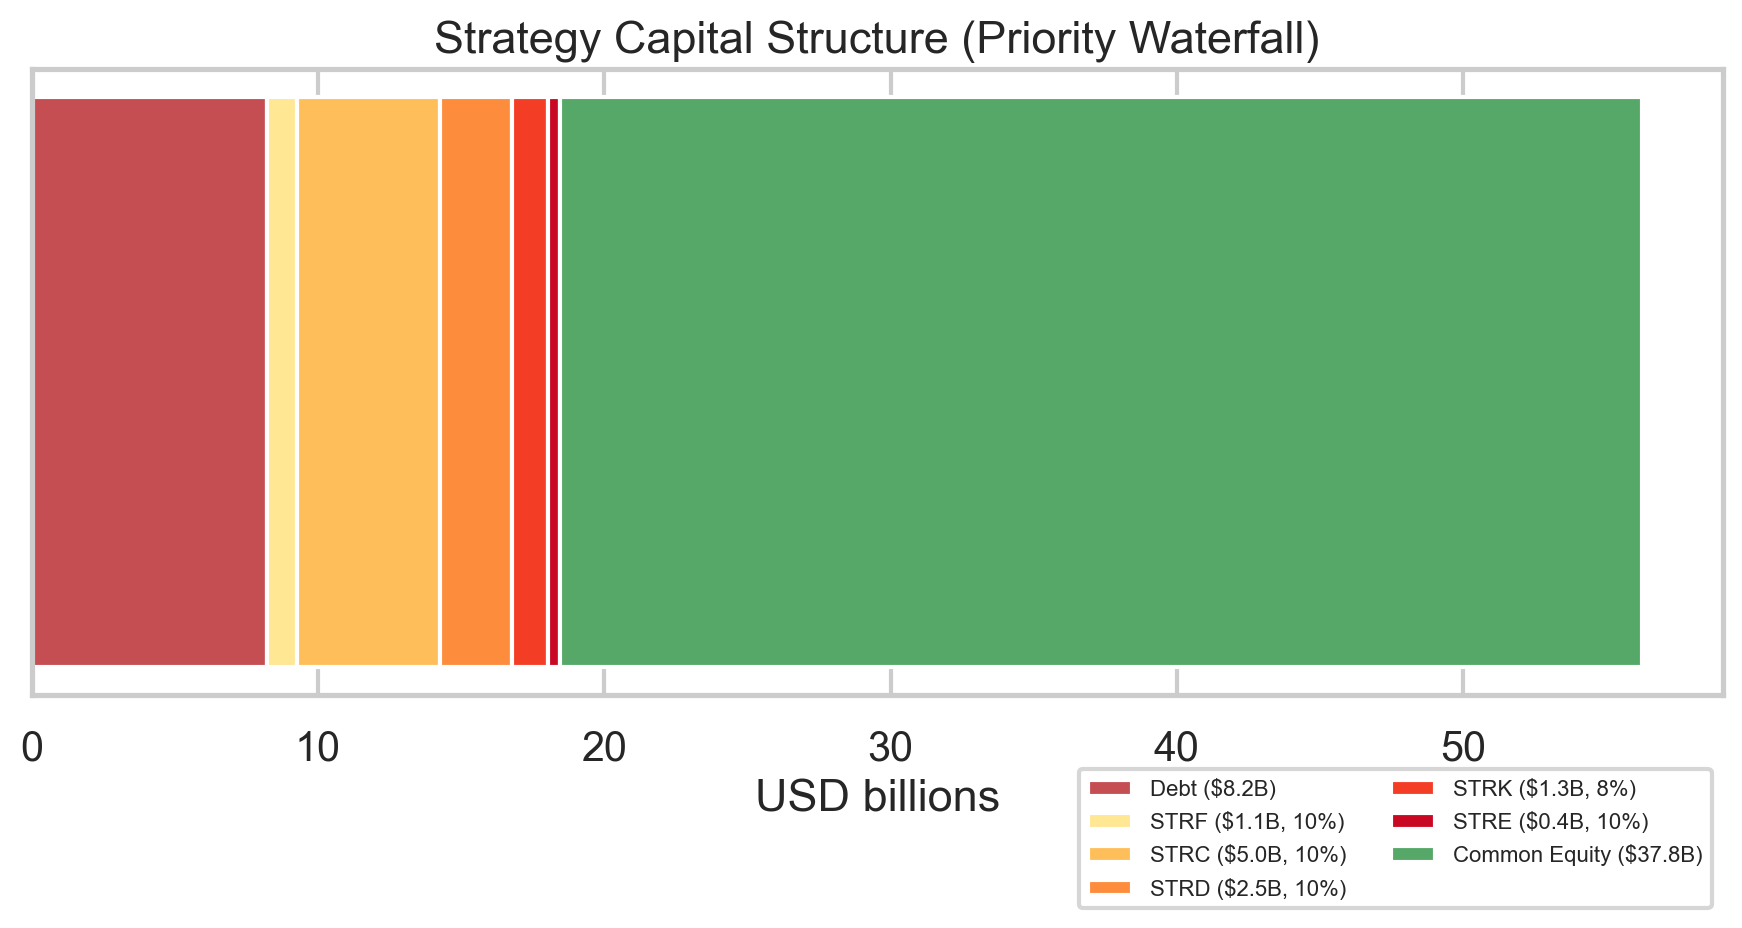
\includegraphics[width=0.7\textwidth]{capital_structure.png}
  \caption{Capital structure priority waterfall (March 2026).
  Debt and preferred constitute \$18.5B in senior claims against
  \$56.3B in BTC assets.}
  \label{fig:capital_structure}
\end{figure}

Figure~\ref{fig:assets_debt_nav} shows the evolution of the capital stack
over the full sample.  BTC assets grew from $\sim$\$3B in early 2021 to
\$56.3B by March~2026, with debt increasing in step-function increments
(convertible issuances) and preferred stock appearing from mid-2025.

\begin{figure}[H]
  \centering
  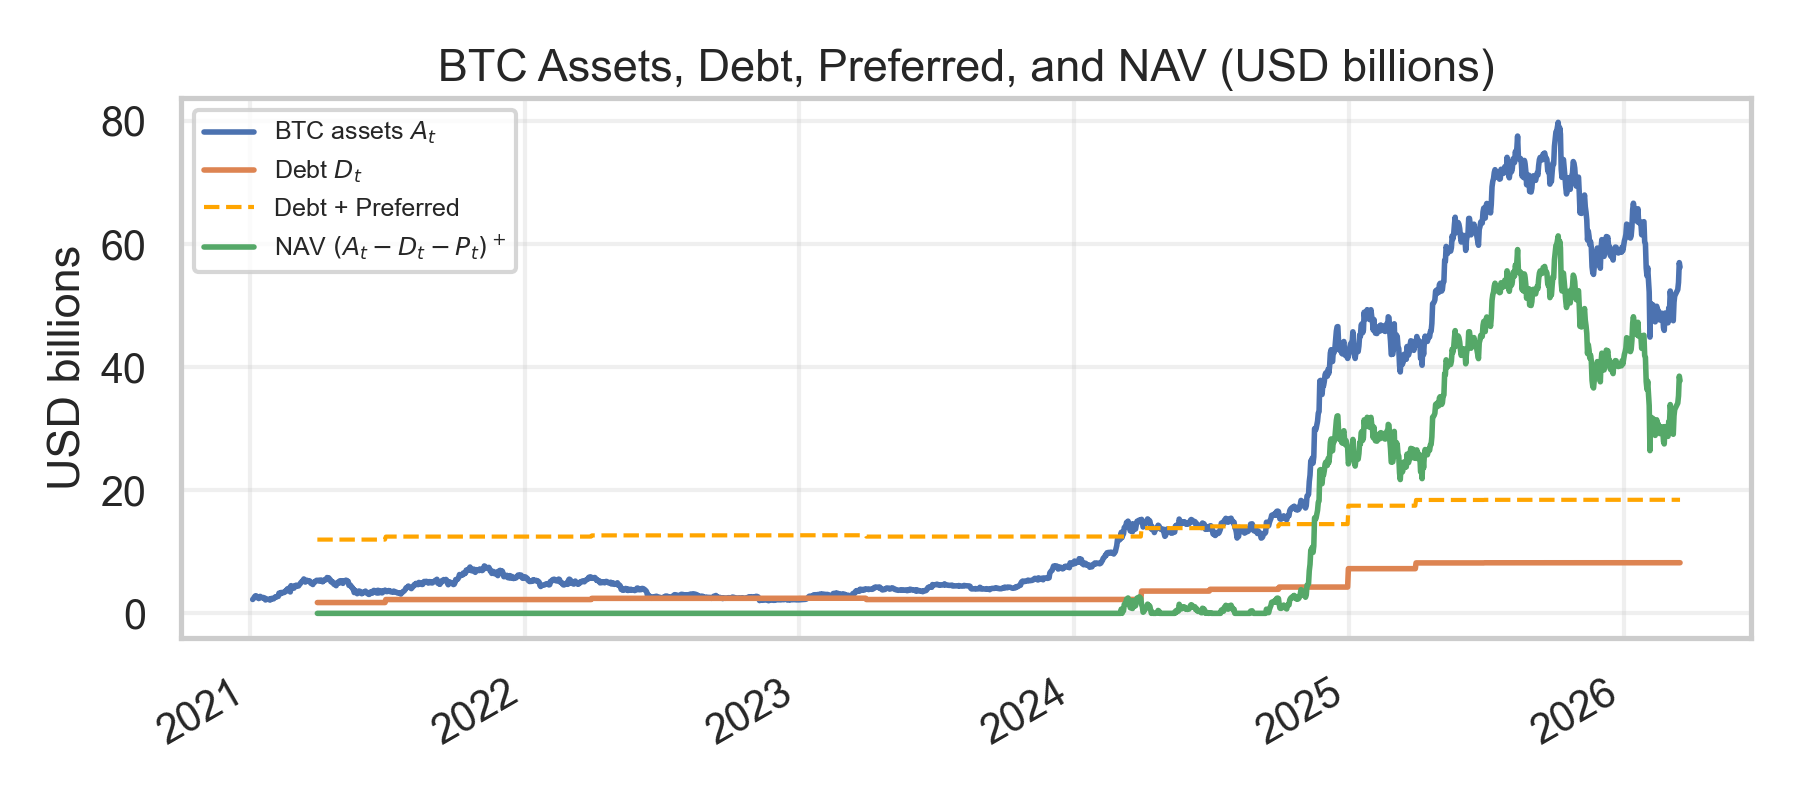
\includegraphics[width=0.85\textwidth]{assets_debt_nav.png}
  \caption{BTC assets, debt, preferred stock, and NAV (2021--2026).}
  \label{fig:assets_debt_nav}
\end{figure}

%=============================================================================
\subsection{Premium Dynamics}\label{sec:premium_dynamics}
%=============================================================================

Figure~\ref{fig:premium_ts} displays the premium time series.  The premium
was relatively stable at 20--25\% through 2021--2024, spiked dramatically
in Q4~2024 (exceeding 200\% during the BTC rally to \$100K+), and has
since decayed toward the current level of 24.2\%.

\begin{figure}[H]
  \centering
  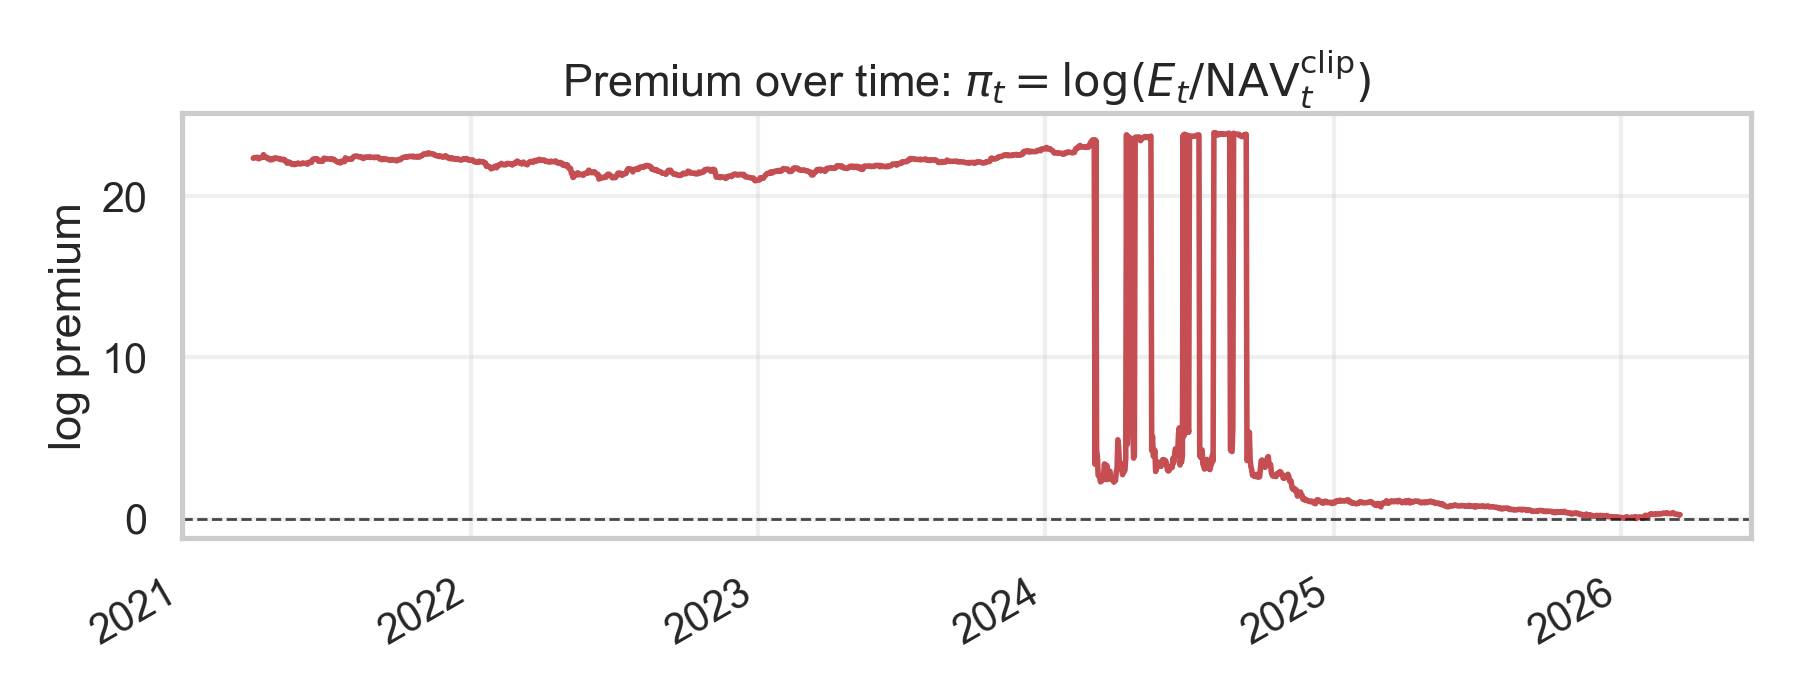
\includegraphics[width=0.85\textwidth]{premium_timeseries.png}
  \caption{Log-premium $\pi_t$ (2021--2026).  The OU long-run mean
  $\hat\theta = 1.08$ reflects the full-sample average including
  the Q4~2024 spike.}
  \label{fig:premium_ts}
\end{figure}

%=============================================================================
\subsection{Leverage and Equity Elasticity}\label{sec:ile_tee}
%=============================================================================

Figure~\ref{fig:ile_tee} shows the ILE and TEE time series.  Both spiked
dramatically in 2024 during periods of high leverage (when NAV was
compressed) and have since stabilised at moderate levels.

\begin{figure}[H]
  \centering
  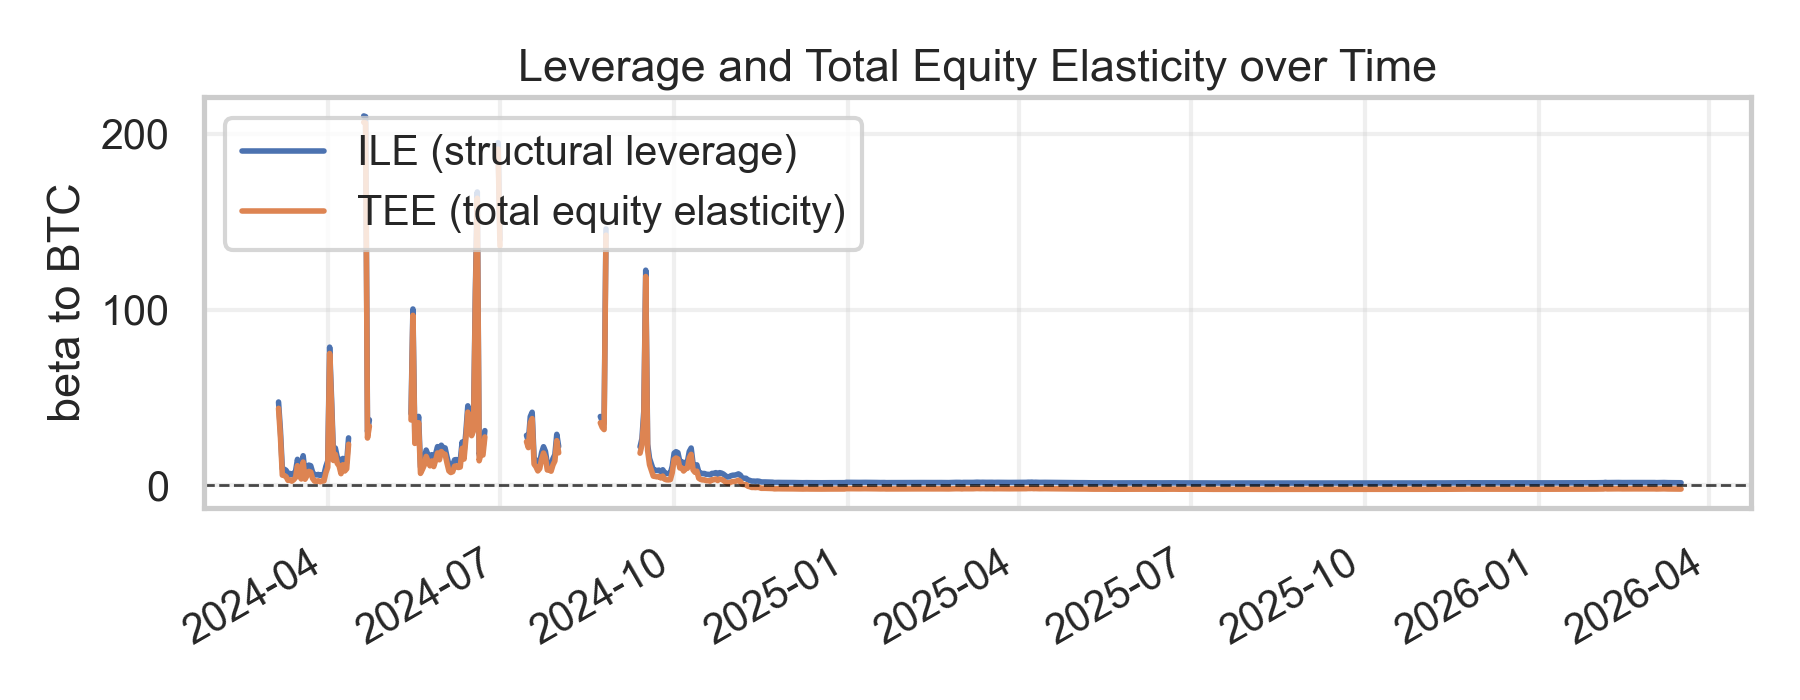
\includegraphics[width=0.85\textwidth]{ile_tee_timeseries.png}
  \caption{ILE (leverage Delta) and TEE (total Delta), 2024--2026.}
  \label{fig:ile_tee}
\end{figure}

%=============================================================================
\subsection{BTC Per Share}\label{sec:btc_per_share}
%=============================================================================

Figure~\ref{fig:btc_per_share} tracks BTC per share over time.  The measure
was stable at $\sim$0.013 BTC/share through 2021--2024, with a
discontinuity at the August~2024 10-for-1 split.  Post-split, the
per-share holding is $\sim$0.0024, reflecting both the split adjustment
and the dilution from preferred stock issuance.

\begin{figure}[H]
  \centering
  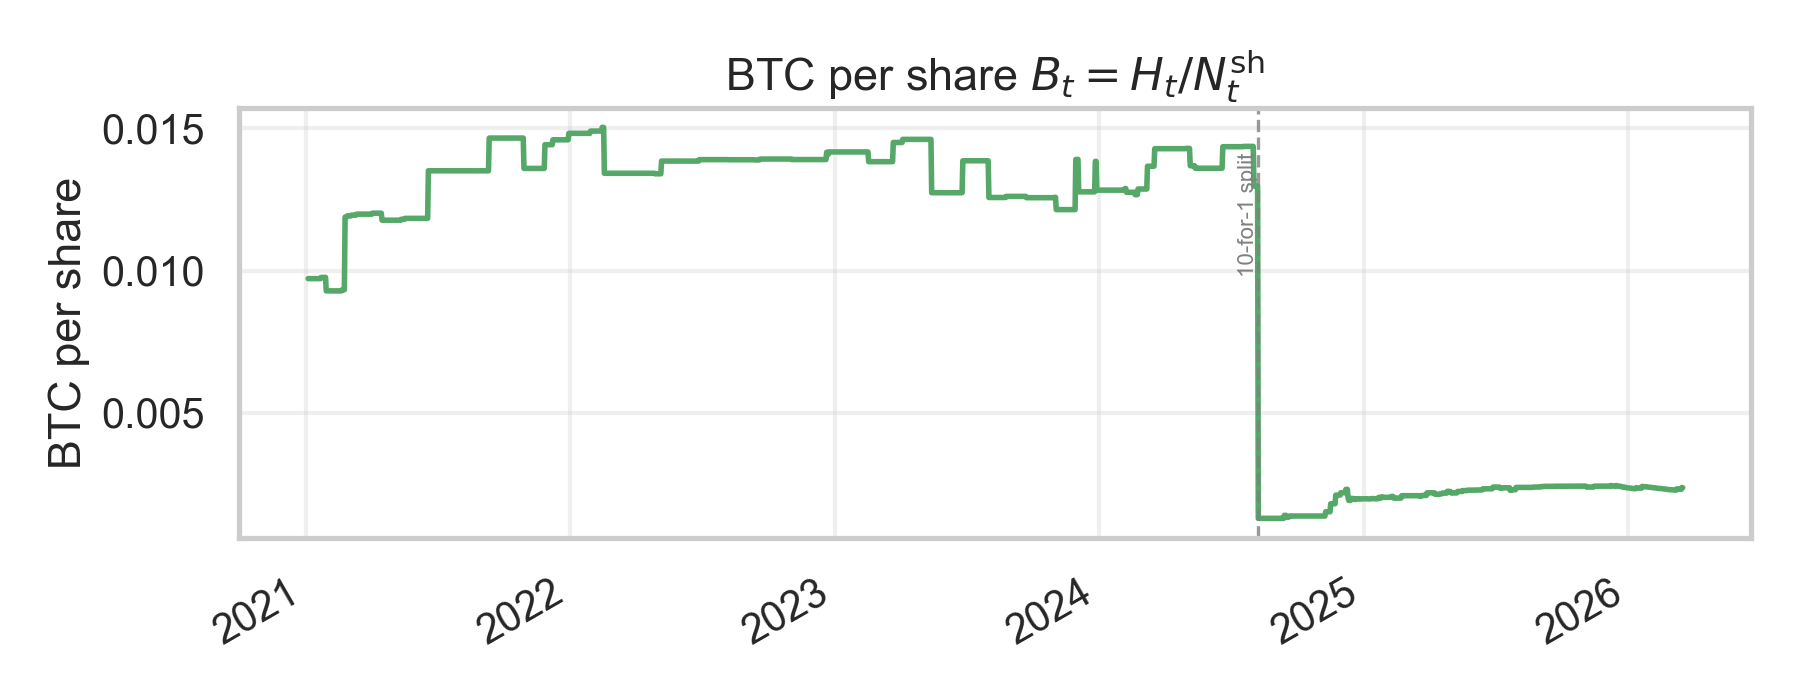
\includegraphics[width=0.85\textwidth]{btc_per_share_timeseries.png}
  \caption{BTC per share (2021--2026).  Vertical line marks the
  10-for-1 stock split (August 8, 2024).}
  \label{fig:btc_per_share}
\end{figure}

%=============================================================================
\subsection{Implied Funding Requirement Distribution}\label{sec:ifrd_results}
%=============================================================================

Figure~\ref{fig:ifrd} shows the Monte Carlo distribution of the three-year
cumulative funding requirement $G_{3\mathrm{y}} = \int_0^3 S_u\,dH_u$
across 5,000 simulated paths.

\begin{figure}[H]
  \centering
  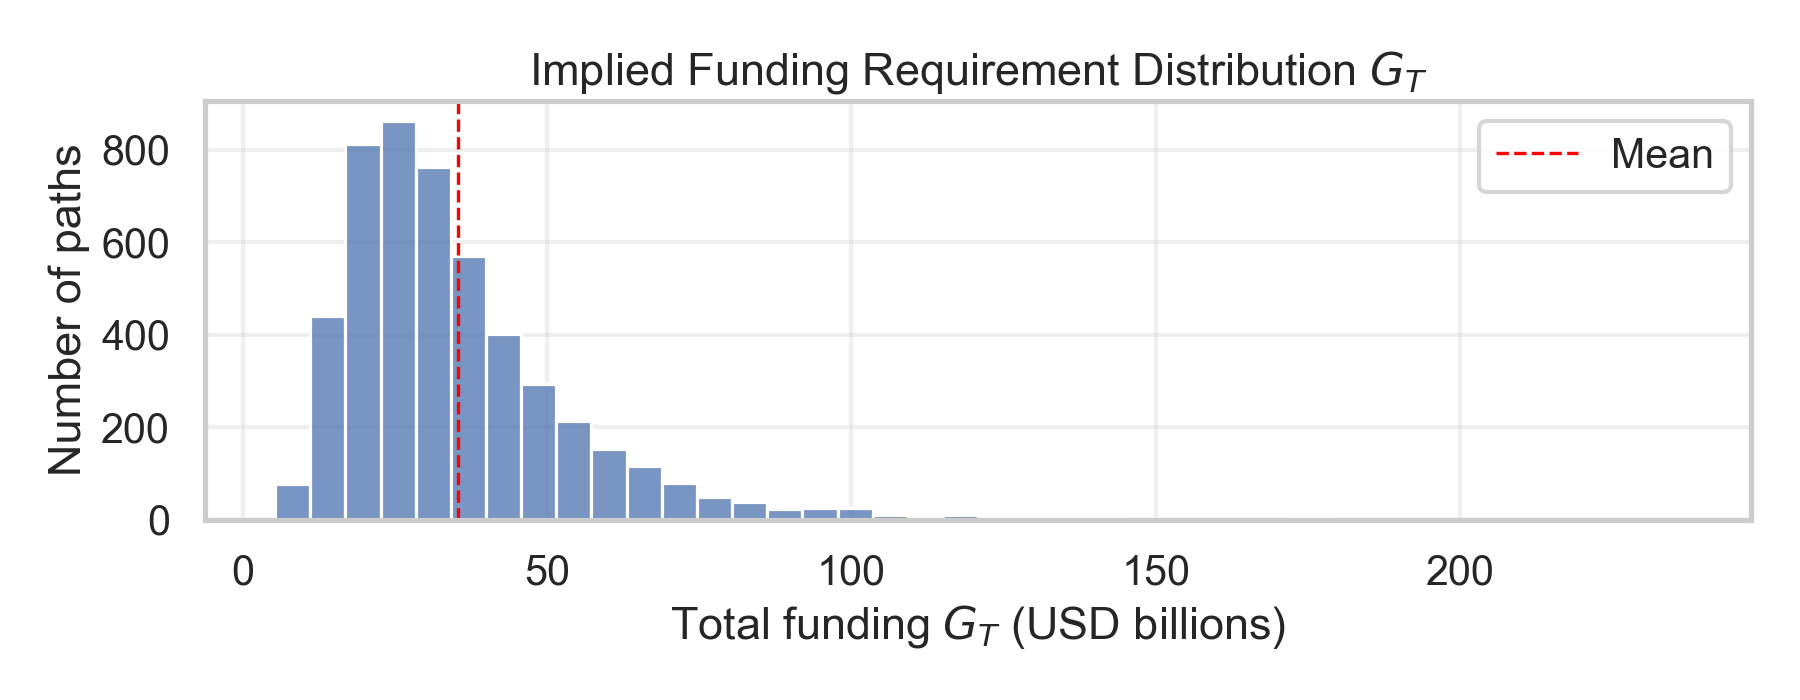
\includegraphics[width=0.7\textwidth]{ifrd_histogram.png}
  \caption{Implied Funding Requirement Distribution (3-year horizon,
  5,000 paths).  Mean: \$35.3B; median: $\sim$\$30B; 95th percentile:
  \$71.8B.}
  \label{fig:ifrd}
\end{figure}

The right-skewed distribution reflects the compounding interaction between
BTC price appreciation and holding growth: in bullish scenarios, both $S_t$
and $dH_t$ increase, producing disproportionately large funding requirements.
The 95th-percentile value of \$71.8B flags the tail scenario where capital
markets must remain extremely accommodative.

%=============================================================================
\subsection{Theory Validation}\label{sec:theory_validation}
%=============================================================================

We assess whether the calibrated values support the theoretical predictions.

\paragraph{Prediction 1: Positive premium from accumulation option.}
The current premium $\pi_0 = 0.242 > 0$ is consistent with
Proposition~\ref{prop:fair_premium}: Strategy has positive issuance
capability (IBGR $= 17.6\%$) and positive NAV, so the accumulation
option has value and the fair premium is positive.

\paragraph{Prediction 2: Premium below steady-state fair value.}
The PMRI of $-0.71$ indicates the premium is below the OU long-run mean
$\theta = 1.08$.  Under the endogenous model, this corresponds to a
mispricing Z-score of $-0.71$ (Definition~\ref{def:zscore}), suggesting
moderate undervaluation---the market is not fully pricing the
accumulation option.

\paragraph{Prediction 3: Optimal financing matches premium regime.}
The ATM accretion threshold is $\log(\mathrm{ILE}_0) = \log(1.488) = 0.397$.
Since $\pi_0 = 0.242 < 0.397$, the model predicts ATM equity issuance is
mildly dilutive.  This matches Strategy's observed shift away from common
equity ATM toward preferred stock issuance in late 2025--early 2026
(Proposition~\ref{prop:optimal_channel}).

\paragraph{Prediction 4: Premium compression dampens reflexivity.}
The negative $\gamma_{\pi S} = -3.60$ yields $\beta_{\mathrm{TOT}} = -2.11$,
implying that the reflexive amplification factor $R_t < 1$
(Proposition~\ref{prop:instability}).  Price impact from Strategy purchases
is \emph{attenuated} rather than amplified at current calibration.  This
is a stabilising regime.

\paragraph{Prediction 5: Adequate survival margin.}
The full-stack distress threshold
$(D_0 + P_0^{\mathrm{liq}})/H_0 = \$18.45\text{B}/761{,}068 = \$24{,}200$
is 67\% below the current BTC price of \$73,909.  The 91.9\% three-year
survival probability (Theorem~\ref{thm:death_spiral}) indicates the
death spiral is a low-probability tail event given current market
conditions.

\paragraph{Prediction 6: Procyclical leverage.}
The theoretical prediction that leverage falls in bull markets and rises in
bear markets (Proposition~\ref{prop:procyclical}) is confirmed by the
ILE time series (Figure~\ref{fig:ile_tee}): ILE spiked during the
2024 drawdown and compressed as BTC recovered.

%!TEX root = ../main.tex

\section{Discussion}\label{sec:discussion}

%=============================================================================
\subsection{Theory Assessment}
%=============================================================================

The endogenous premium model provides a coherent explanation for Strategy's
persistent NAV premium.  The core insight---that the premium is the present
value of an accumulation option---resolves the apparent anomaly: unlike a
closed-end fund discount driven by sentiment or agency costs, the premium
reflects genuine economic value created by the ability to issue equity above
NAV and purchase BTC accretively.

The model's predictions align well with calibrated data across six
dimensions (Section~\ref{sec:theory_validation}): positive premium from
accumulation capability, premium below steady-state implying positive carry,
financing channel selection matching the premium regime, dampened reflexivity
from premium compression, adequate survival margin, and procyclical leverage.

The fixed-point equation~\eqref{eq:pi_star_closed} provides a quantitative
tool for premium assessment.  At steady state, the fair premium is determined
by four fundamentals: BTC volatility $\sigma_S$ (positive vega), issuance
intensity $\alpha_N$ (moneyness), leverage $\ell$ (negative effect), and
discount rate $r$ (negative rho).  Changes in any of these fundamentals
shift the equilibrium, with the comparative statics providing directional
guidance.

%=============================================================================
\subsection{Where Is Strategy Currently?}
%=============================================================================

The indicator dashboard places Strategy in the ``MSTR dominates'' quadrant
of the regime map (Corollary~\ref{cor:regime_map}): IBGR is positive
(17.6\%) and PMRI is negative ($-0.71$).  The accumulation option is in the
money, the premium is underpriced relative to its long-run equilibrium,
and leverage is moderate ($\mathrm{ILE} = 1.49 < 2$).

However, several factors warrant caution:
\begin{itemize}
  \item The current premium ($\pi_0 = 0.242$) is below the ATM accretion
    threshold ($\pi^*_{\mathrm{ATM}} = 0.397$), meaning common equity
    issuance is currently mildly dilutive.  Strategy must rely on
    preferred stock and convertible debt to fund BTC purchases---channels
    with effective costs of 10--12.5\%.
  \item The preferred dividend burden of \$977M/year is a fixed obligation
    regardless of BTC price.  While the dividend coverage ratio is
    comfortable at 49$\times$, a sustained BTC decline to \$15,000--\$20,000
    would bring the leverage spiral condition
    (Corollary~\ref{cor:leverage_spiral}) into play.
  \item The 91.9\% three-year survival probability, while reassuring,
    implies an 8.1\% probability of NAV breach---non-trivial for a
    single-asset vehicle.
\end{itemize}

The critical near-term question is whether the premium recovers above the
ATM threshold, re-enabling the cheapest financing channel.  If BTC
appreciates significantly and the premium expands, the flywheel can
re-engage.  If the premium continues to compress, Strategy faces increasing
reliance on expensive preferred financing, degrading the capital structure
toward the tipping point of Theorem~\ref{thm:three_equilibria}.

%=============================================================================
\subsection{Implications for Investors}
%=============================================================================

\paragraph{MSTR vs.\ ETF.}
At the current calibration point, the indicators favour MSTR over a spot
BTC ETF for investors with sufficient risk tolerance:
\begin{itemize}
  \item Positive carry from $\mathrm{PMRI} < 0$ (expected premium
    expansion).
  \item Active accumulation option (IBGR $> 0$).
  \item Moderate leverage providing amplified upside.
\end{itemize}
However, the ETF is preferable for investors seeking pure BTC exposure
without the embedded risks of the capital structure, particularly given
the negative TEE (equity moving inversely to BTC at the margin).

\paragraph{Signal monitoring.}
The regime map provides actionable signals:
\begin{itemize}
  \item \textbf{PMRI crossing zero} signals the transition from
    positive to negative carry---the premium is now overpriced relative
    to fundamentals.
  \item \textbf{IBGR approaching zero} signals the flywheel is stalling
    ---accumulation is no longer accretive.
  \item \textbf{ILE exceeding 2} signals excessive leverage and
    elevated tail risk.
  \item \textbf{DCR falling below 10$\times$} signals preferred dividend
    sustainability concerns.
\end{itemize}

%=============================================================================
\subsection{Optimal Capital Structure Prescriptions}
%=============================================================================

The analysis yields concrete prescriptions for Strategy's financing:
\begin{enumerate}
  \item \textbf{Resume ATM when $\pi_t > 0.40$:} This is the accretion
    threshold at current leverage.  ATM issuance is the cheapest channel
    and should be used aggressively above this level.
  \item \textbf{Limit preferred issuance:} Each additional preferred
    series increases the dividend burden and the ATM accretion threshold
    ($\pi^*_{\mathrm{ATM}} = \log(\mathrm{ILE})$ rises with
    $P^{\mathrm{liq}}$).  The current \$977M annual dividend is already
    a material fixed cost.
  \item \textbf{Maintain cash buffer:} The \$2.25B cash reserve provides
    2.5 years of preferred dividend coverage in a zero-BTC-liquidation
    scenario.  This buffer is essential for surviving temporary drawdowns
    without forced sales.
  \item \textbf{Minimise WACBA:} Financing decisions should target the
    lowest WACBA given premium and leverage constraints, shifting
    channels as $\pi_t$ fluctuates.
\end{enumerate}

%=============================================================================
\subsection{Systemic Risk}
%=============================================================================

Strategy's success has catalysed corporate BTC adoption: over 70 public
companies now hold Bitcoin on balance sheet.  The market impact analysis
(Section~\ref{sec:market_impact_theory}) highlights two systemic
considerations:

\begin{enumerate}
  \item \textbf{Concentration risk:} Strategy holds 3.84\% of circulating
    BTC supply.  A forced liquidation at the full-stack distress threshold
    (\$24,200) would involve selling up to 761,068~BTC, roughly 30 days
    of average trading volume.  The price impact of such a sale, using
    Kyle lambda estimates, would be devastating.
  \item \textbf{Contagion:} If aggregate corporate holdings reach
    10--15\% of circulating supply, the contagion cascade mechanism
    (Theorem~\ref{thm:contagion}) becomes material.  A BTC decline that
    triggers one firm's distress threshold could propagate through
    correlated forced sales.
\end{enumerate}

The asymptotic stability result (Corollary~\ref{cor:asymptotic}) provides
a counterpoint: as BTC market depth grows ($2g_S + g_V > g_E$), the
reflexive feedback naturally weakens.  The question is whether market
maturation outpaces corporate adoption.

%=============================================================================
\subsection{Limitations and Future Work}
%=============================================================================

\paragraph{Limitations.}
\begin{enumerate}
  \item \emph{Physical measure:} We work under $\mathbb{P}$ throughout.
    A risk-neutral ($\mathbb{Q}$) formulation would enable derivative
    pricing and arbitrage-free valuation.
  \item \emph{Constant parameters:} The OU calibration assumes
    time-invariant $\kappa$, $\theta$, $\sigma_\pi$.  Regime-switching
    or time-varying parameters may better capture the structural
    break around the Q4~2024 premium spike.
  \item \emph{Single-firm focus:} Calibration is specific to Strategy.
    Generalisation to other BTC treasury vehicles requires
    firm-specific parameter estimation.
  \item \emph{Preferred stock modelling:} We treat preferred stock as a
    fixed obligation (liquidation value plus dividends).  The embedded
    call provisions, conversion optionality (STRK), and variable-rate
    features (STRC) introduce additional complexity not fully captured.
  \item \emph{Market impact estimation:} The Kyle lambda parameter
    $\eta$ is not directly estimated from our data.  We rely on
    literature estimates for illustrative analysis.
\end{enumerate}

\paragraph{Future work.}
Natural extensions include: (i)~risk-neutral pricing of the accumulation
option using derivatives data; (ii)~regime-switching models for $\kappa$
and $\theta$; (iii)~cross-sectional estimation across multiple BTC treasury
vehicles; (iv)~structural estimation of the feedback gain $G$ from
high-frequency issuance-price data; and (v)~welfare analysis of corporate
BTC adoption under the contagion cascade framework.

%!TEX root = ../main.tex

\section{Conclusion}\label{sec:conclusion}

We develop a structural theory of endogenous premium formation for Bitcoin
treasury vehicles.  The NAV premium is the market value of a perpetual
accumulation option---the right to issue equity above NAV and purchase BTC
accretively.  The fair premium satisfies a fixed-point equation whose
steady-state closed form connects to the Black--Scholes formula, linking
the premium to BTC volatility, issuance capability, leverage, and discount
rates.

The reflexive feedback between premium and accumulation generates multiple
equilibria: a high-premium flywheel, an unstable tipping point, and a
low-premium death spiral, connected by saddle-node bifurcations with
hysteresis.  We reinterpret five structural indicators as the option Greeks
of the accumulation claim and derive optimal capital structure rules
governing the transition among financing channels.

Calibrating to Strategy (MSTR) through March~2026, we find the current
premium of 24.2\% sits below the OU long-run mean ($\text{PMRI} = -0.71$),
implying positive carry and an underpriced accumulation option.  Leverage is
moderate ($\mathrm{ILE} = 1.49$), the flywheel is active
($\mathrm{IBGR} = 17.6\%$), and three-year survival probability is 91.9\%.
The framework provides a unified lens for valuation, risk monitoring, and
vehicle selection in the emerging landscape of corporate Bitcoin treasury
strategies.


\newpage
\bibliographystyle{plainnat}
\bibliography{references}

\end{document}
